\documentclass{beamer}

\mode<presentation>{
  % \useinnertheme{rectangles}
  \useoutertheme{infolines}
  % \usecolortheme{crane}
  % \usecolortheme{rose}
}
%% Pre-amble - commonly defined macros.

%% Packages
\usepackage{amsmath}
\usepackage{amsfonts}
\usepackage{amssymb}
\usepackage{amsbsy}
\usepackage{isomath}
\usepackage{amsthm}
\usepackage{dsfont}
%%\usepackage{theorem}
\usepackage{algorithm}
\usepackage{algorithmicx}
\usepackage{algpseudocode}
\usepackage{mathrsfs}
\usepackage{epsfig}
\usepackage{subcaption}
\usepackage{makeidx} 
\usepackage{colortbl}
\usepackage{enumerate}
\usepackage{multirow}
\usepackage{listings}
\usepackage{pgfplots}
\newlength\fheight
\newlength\fwidth
\only<presentation>{
\setlength\fheight{0.5\columnwidth}
\setlength\fwidth{0.5\columnwidth}
}
\only<article>{
\setlength\fheight{0.25\textwidth}
\setlength\fwidth{0.25\textwidth}
}
\usepackage[sort&compress,comma,super]{natbib}
\def\newblock{} % To avoid a compilation error about a function \newblock undefined
\usepackage{hyperref}

\setbeamertemplate{theorems}[numbered] 
\mode<presentation>{
\theoremstyle{plain}
\newtheorem{assumption}{Assumption}
\theoremstyle{definition}
\newtheorem{exercise}{Exercise}
\theoremstyle{remark}
\newtheorem{remark}{Remark}
}

\numberwithin{equation}{section} 
\mode<article>{
\theoremstyle{plain}
%    \newtheorem{assumption}{Assumption}[section]
\newtheorem{lemma}{Lemma}[section]
\newtheorem{theorem}{Theorem}[section]
\newtheorem{corollary}{Corollary}[section]
\theoremstyle{definition}
\newtheorem{definition}{Definition}[section]
\theoremstyle{remark}
\newtheorem{remark}{Remark}[section]

%\theoremstyle{plain} \newtheorem{remark}{Remark}[section]
%\theoremstyle{plain} \newtheorem{definition}{Definition}[section]
\theoremstyle{plain} \newtheorem{assumption}{Assumption}[section]

%%% Examples %%%%
\newtheoremstyle{example}  % Name
{1em}       % Space above 
{1em}       % Space below
{\small}      % Body font
{}          % Indent amount 
{\scshape}  % Theorem head font
{.}         % Punctuation after theorem head
{.5em}      % Space after theorem head
{}          % Theorem head spec
\theoremstyle{example}
\newtheorem{example}{Example}
\newtheorem{exercise}{Exercise}

\usepackage{framed}
\renewenvironment{block}[1]
{\framed \par \textbf{#1} \newline}
{\par \endframed}

\renewenvironment{exampleblock}[1]
{\framed \par \textit{#1} \newline \bigskip}
{\par \endframed}

\renewenvironment{alertblock}[1]
{\framed \par \textit{\textbf{#1}} \newline \hrule \bigskip}
{\par \endframed}
}


%\theoremstyle{plain} \newtheorem{conjecture}{Conjecture}[section]
%\theoremstyle{plain} \newtheorem{theorem}{Theorem}[section]
%\theoremstyle{plain} \newtheorem{proposition}{Proposition}[section]
%\theoremstyle{plain} \newtheorem{lemma}{Lemma}[section]
%\theoremstyle{plain} \newtheorem{corollary}{Corollary}[section]


%\newenvironment{proof}[1][Proof]{\begin{trivlist}
%\item[\hskip \labelsep {\bfseries #1}]}{\end{trivlist}}
%\newcommand{\qed}{\nobreak \ifvmode \relax \else
%      \ifdim\lastskip<1.5em \hskip-\lastskip
%      \hskip1.5em plus0em minus0.5em \fi \nobreak
%      \vrule height0.5em width0.5em depth0.25em\fi}

\newcommand \indexmargin[1] {\marginpar{\emph{#1}}\index{#1}}
\newcommand \marginref[2] {\marginpar{\emph{#1}}\emph{#1}\index{#2}}
\newcommand \emindex[1] {\emph{#1}\marginpar{\emph{#1}}\index{#1}}


\newcommand \E {\mathop{\mbox{\ensuremath{\mathbb{E}}}}\nolimits}
\newcommand \hE {\hat{\mathop{\mbox{\ensuremath{\mathbb{E}}}}\nolimits}}
\renewcommand \Pr {\mathop{\mbox{\ensuremath{\mathbb{P}}}}\nolimits}
\newcommand \given {\mathrel{|}}
\newcommand \gvn {|}
\newcommand \eq {{=}}


%% Special characters
\newcommand\Reals {{\mathbb{R}}}
\newcommand\Naturals {{\mathbb{N}}} 
\newcommand\Simplex {\mathbold{\Delta}}

\newcommand \FB {{\mathfrak{B}}}
\newcommand \FD {{\mathfrak{D}}}
\newcommand \FF {{\mathfrak{F}}}
\newcommand \FM {{\mathfrak{M}}}
\newcommand \FK {{\mathfrak{K}}}
\newcommand \FJ {{\mathfrak{J}}}
\newcommand \FL {{\mathfrak{L}}}
\newcommand \FO {{\mathfrak{O}}}
\newcommand \FS {{\mathfrak{S}}}
\newcommand \FT {{\mathfrak{T}}}
\newcommand \FP {{\mathfrak{P}}}
\newcommand \FR {{\mathfrak{R}}}


\newcommand \CA {{\mathcal{A}}}
\newcommand \CB {{\mathcal{B}}}
\newcommand \CC {{\mathcal{C}}}
\newcommand \CD {{\mathcal{D}}}
\newcommand \CE {{\mathcal{E}}}
\newcommand \CF {{\mathcal{F}}}
\newcommand \CG {{\mathcal{G}}}
\newcommand \CH {{\mathcal{H}}}
\newcommand \CJ {{\mathcal{J}}}
\newcommand \CL {{\mathcal{L}}}
\newcommand \CM {{\mathcal{M}}}
\newcommand \CN {{\mathcal{N}}}
\newcommand \CO {{\mathcal{O}}}
\newcommand \CP {{\mathcal{P}}}
\newcommand \CQ {{\mathcal{Q}}}
\newcommand \CR {{\mathcal{R}}}
\newcommand \CS {{\mathcal{S}}}
\newcommand \CT {{\mathcal{T}}}
\newcommand \CU {{\mathcal{U}}}
\newcommand \CV {{\mathcal{V}}}
\newcommand \CW {{\mathcal{W}}}
\newcommand \CX {{\mathcal{X}}}
\newcommand \CY {{\mathcal{Y}}}
\newcommand \CZ {{\mathcal{Z}}}

\newcommand \BA {{\mathbb{A}}}
\newcommand \BI {{\mathbb{I}}}
\newcommand \BS {{\mathbb{S}}}

\newcommand \bx {{\mathbf{x}}}
\newcommand \by {{\mathbf{y}}}
\newcommand \bu {{\mathbf{u}}}
\newcommand \bw {{\mathbf{w}}}
\newcommand \ba {{\mathbf{a}}}
\newcommand \bz {{\mathbf{z}}}
\newcommand \bat {{\mathbf{a}_t}}
\newcommand \bh {{\mathbf{h}}}
\newcommand \bo {{\mathbf{o}}}
\newcommand \bp {{\mathbf{p}}}
\newcommand \bs {{\mathbf{s}}}
\newcommand \br {{\mathbf{r}}}

\newcommand \SA {\mathscr{A}}
\newcommand \SB {\mathscr{B}}
\newcommand \SC {\mathscr{C}}
\newcommand \SF {\mathscr{F}}
\newcommand \SG {\mathscr{G}}
\newcommand \SH {\mathscr{H}}
\newcommand \SJ {\mathscr{J}}
\newcommand \SL {\mathscr{L}}
\newcommand \SP {\mathscr{P}}
\newcommand \SR {\mathscr{R}}
%%\newcommand \SS {\mathscr{S}}
\newcommand \ST {\mathscr{T}}
\newcommand \SU {\mathscr{U}}
\newcommand \SV {\mathscr{V}}
\newcommand \SW {\mathscr{W}}

\newcommand \hM {\widehat{M}}

\newcommand \KL[2] {\mathbb{D}\left( #1 \| #2 \right)}


%\newcommand \p {\partial}

\newcommand \then{\Rightarrow}
\newcommand \defn {\mathrel{\triangleq}}
%\newcommand \StateSet {{\CQ}}


%% Commands

\newcommand \argmax{\mathop{\rm arg\,max}}
\newcommand \argmin{\mathop{\rm arg\,min}}
\newcommand \dtan{\mathop{\rm dtan}}
\newcommand \sgn{\mathop{\rm sgn}}
\newcommand \trace{\mathop{\rm tr}}

\newcommand \onenorm[1]{\left\|#1\right\|_1}
\newcommand \pnorm[2]{\left\|#1\right\|_{#2}}
\newcommand \inftynorm[1]{\left\right\|#1\|_\infty}
\newcommand \norm[1]{\left\|#1\right\|}

%%\newcommand \defn {\triangleq}
%%\newcommand \defn {\equiv}
%%\newcommand \defn {\coloneq}
%%\newcommand \defn {\stackrel{\text{\tiny def}}{=}}
%%\newcommand \defn {\stackrel{\text{def}}{\hbox{\equalsfill}}}

\DeclareMathAlphabet{\mathpzc}{OT1}{pzc}{m}{it}

\newcommand \Normal {\mathop{\mathpzc{N}}\nolimits}
\newcommand \Poisson {\mathop{\mathpzc{Poisson}}\nolimits}
\newcommand \Multinomial {\mathop{\mathpzc{Multinomial}}\nolimits}
\newcommand \Dirichlet {\mathop{\mathpzc{Dirichlet}}\nolimits}
\newcommand \Student {\mathop{\mathpzc{Student}}\nolimits}
\newcommand \Bernoulli {\mathop{\mathpzc{Bernoulli}}\nolimits}
\newcommand \BetaDist   {\mathop{\mathpzc{Beta}}\nolimits}
\newcommand \Singular   {\mathop{\mathpzc{D}}\nolimits}
\newcommand \GammaDist {\mathop{\mathpzc{Gamma}}\nolimits}
\newcommand \Softmax{\mathop{\mathpzc{Softmax}}\nolimits}
\newcommand \Exp{\mathop{\mathpzc{Exp}}\nolimits}
\newcommand \Uniform{\mathop{\mathpzc{Unif}}\nolimits}
\newcommand \Laplace {\mathop{\mathpzc{Laplace}}\nolimits}

\newcommand \Param {\Theta}
\newcommand \param {\theta}
\newcommand \vparam {\vectorsym{\theta}}
\newcommand \mparam {\matrixsym{\Theta}}
\newcommand \Hyperparam {\Phi}
\newcommand \hyperparam {\phi}
\newcommand \family {\mathcal{F}}
\newcommand{\ie}{\emph{i.e.}\xspace}
\newcommand{\eg}{\emph{e.g.}\xspace}
\newcommand{\etal}{\emph{et al.}\xspace}
\newcommand{\constg}{}
\newcommand{\Bel}{\Xi}
\newcommand \Bay {\ensuremath{\mathscr{B}}}
\newcommand \Adv {\ensuremath{\mathscr{A}}}


\newcommand \Borel[1] {\FF(#1)}
\newcommand \Probs[1] {\FM(#1)}


\newcommand \pol {\pi}
\newcommand \Pol {\Pi}
\newcommand \mdp {\mu}
\newcommand \MDP {\CM}
\newcommand \meanMDP {{\bar{\mdp}_\xi}}

\newcommand {\msqr} {\vrule height0.33cm width0.44cm}
\newcommand {\bsqr} {\vrule height0.55cm width0.66cm}

\newcommand\ind[1]{\mathop{\mbox{\ensuremath{\mathbb{I}}}}\left\{#1\right\}}
\newcommand\Ind{\mbox{\bf{I}}}

\newcommand\dd{\,\mathrm{d}}

\newcommand \seq[2]{#1^{#2}}
\newcommand \pseq[3]{#1_{#2}^{#3}}
\newcommand \sam[2]{#1^{(#2)}}
\newcommand \transpose[1] {#1^\top}
\newcommand\set[1] {\left\{#1\right\}}
\newcommand\tuple[1] {\left\langle #1\right\rangle}
\newcommand\cset[2] {\left\{#1 ~\middle|~ #2\right\}}
\newcommand \ceil[1]{\left\lceil #1 \right\rceil}





\newcommand{\indep}{\mathrel{\text{\scalebox{1.07}{$\perp\mkern-10mu\perp$}}}}


\newcommand \eqlike {\eqsim}
\newcommand \gtlike {\succ}
\newcommand \ltlike {\prec}
\newcommand \gelike {\succsim}
\newcommand \lelike {\precsim}

\newcommand \eqpref {\eqsim^*}
\newcommand \gtpref {\succ^*}
\newcommand \ltpref {\prec^*}
\newcommand \gepref {\succsim^*}
\newcommand \lepref {\precsim^*}

\newcommand \util {U}
\newcommand \BUtil {U^*}
\newcommand \MUtil {\matrixsym{U}}
\newcommand \risk {\sigma}
\newcommand \Brisk {\sigma^*}
\newcommand \Loss {\ell}
\newcommand \Regret {L}
\newcommand \regret {\ell}
\newcommand \Reward {\SR}
\newcommand \reward {r}
\newcommand \vreward {\vectorsym{r}}
\newcommand \Rew {\rho}
\newcommand \outcome {\omega}
\newcommand \Outcome {\Omega}
\newcommand \act {a}
\newcommand \Act {\CA}
\newcommand \decision {a}
\newcommand \Decision {\mathcal{A}}
\newcommand \dec {\delta}
\newcommand \Dec {\mathscr{D}}


\newcommand {\MH} {\matrixsym{H}}

\newcommand \alg {\lambda}
\newcommand \Alg {\Lambda}
\newcommand \KNN {\textsc{k-NN}}

\newcommand \model {\mu}
\newcommand \MAP {\model_{\textrm{MAP}}}
\newcommand \Model {\CM}
\newcommand \Datasets {\CD}
\newcommand \Data {D}
\newcommand \Training {D_T}
\newcommand \Holdout {D_H}
\newcommand \Testing {D^*}
\newcommand \error {\epsilon}
\newcommand \obs {x}
\newcommand \Obs {\CX}
\newcommand \Att {\CA}
\newcommand \att {a}
\newcommand \attv {v}
\newcommand \Attv {\CV}
\newcommand \cls {y}
\newcommand \Cls {\CY}
\newcommand \Entropy {\mathbb{H}}
\newcommand \Gain {\mathbb{G}}


\newcommand \IDThree {\texttt{ID3}}

\newcommand \nactions {A}
\newcommand \nclasses {C}
\newcommand \nstates{S}
\newcommand \nobservations {N}
\newcommand \ndata{T}

\newcommand \figwidth {0.6\textwidth}
\newcommand \figheight {0.4\textwidth}

\newcommand \eye {\matrixsym{I}}
\newcommand \MA {\matrixsym{A}}
\newcommand \MX {\matrixsym{X}}
\newcommand \MY {\matrixsym{Y}}
\newcommand \MB {\matrixsym{B}}
\newcommand \MV {\matrixsym{V}}
\newcommand \MW {\matrixsym{W}}
\newcommand \MP {\matrixsym{P}}
\newcommand \vg {\vectorsym{\gamma}}
\newcommand \vp {\vectorsym{p}}
\newcommand \vs {\vectorsym{s}}
\newcommand \vx {\vectorsym{x}}
\newcommand \vr {\vectorsym{r}}
\newcommand \vm {\vectorsym{m}}
\newcommand \vb {\vectorsym{b}}
\newcommand \vt {\vectorsym{\theta}}

\newcommand \pn[1] {\vx_{[#1]}}

\newcommand \basis {f}
\newcommand \bel {\xi}
\newcommand \hyper {\omega}
\newcommand \mbel {\bel^D}
\newcommand \pbel {\bel^C}

\newcommand \pmean {\matrixsym{M}}
\newcommand \pcov {\matrixsym{C}}
\newcommand \pwish {\matrixsym{W}}
\newcommand \porder {n}

\newcommand \Syx {\matrixsym{\Sigma}_{yx}}
\newcommand \Sxx {\matrixsym{\Sigma}_{xx}}
\newcommand \Syy {\matrixsym{\Sigma}_{yy}}
\newcommand \Symx {\matrixsym{\Sigma}_{y\mid x}}

\newcommand \trans {\matrixsym{P}}
\newcommand \ident {\matrixsym{I}}

\newcommand \noise {\vectorsym{\varepsilon}}

\newcommand \pt {p_t}


\newcommand \CSet {G}
\newcommand \Parent[1] {\mathfrak{P}(#1)}
\newcommand \Children[1] {\mathfrak{C}(#1)}
\newcommand \Ancestors[1] {\mathfrak{A}(#1)}
\newcommand \Descendants[1] {\mathfrak{D}(#1)}
\newcommand \metric[2] {\nu(#1, #2)}
\newcommand \zooming {\zeta}
\newcommand \depth[1] {d(#1)}

\newcommand \sensitivity[1] {\mathbb{L}\left(#1\right)}
\newcommand \disc {\gamma}
\newcommand \Value {V}
\newcommand \val {\vectorsym{v}}
\newcommand \Vals {\mathcal{V}}
\newcommand \qval {\vectorsym{q}}
\newcommand \Qvals {\mathcal{Q}}
\newcommand \blm {\mathscr{L}}
\newcommand \tdm {\mathscr{D}}
\newcommand \pim {\mathscr{B}}



\newcommand \dist[2]{D\left(#1 ~\middle\|~ #2\right)}

\newcommand \Ae {A_\epsilon^\hist}

\newcommand \lrdist[2]{d_{lr}(#1, #2)}
\newcommand \xdistChar{\rho}
\newcommand \xdist[2]{\xdistChar(#1, #2)}
\newcommand \pdist[2]{\kappa(#1, #2)}
\newcommand{\constScale}{\omega}
\newcommand{\constScaleB}{\kappa}

\newcommand \fields[1]{\sigma(#1)}

\newcommand \hist {h}

\newcommand \abs[1] {\left|#1\right|}

\newcommand{\errorband}[5][]{ % x column, y column, error column, optional argument for setting style of the area plot
\pgfplotstableread[col sep=comma, skip first n=2]{#2}\datatable
% Lower bound (invisible plot)
\addplot [draw=none, stack plots=y, forget plot] table [
x={#3},
y expr=\thisrow{#4}-\thisrow{#5}
] {\datatable};

% Stack twice the error, draw as area plot
\addplot [draw=none, fill=gray!40, stack plots=y, area legend, #1] table [
x={#3},
y expr=2*\thisrow{#5}
] {\datatable} \closedcycle;

% Reset stack using invisible plot
\addplot [forget plot, stack plots=y,draw=none] table [x={#3}, y expr=-(\thisrow{#4}+\thisrow{#5})] {\datatable};
}


%%% macros to make things smalller
% For comparison, the existing overlap macros:
% \def\llap#1{\hbox to 0pt{\hss#1}}
% \def\rlap#1{\hbox to 0pt{#1\hss}}
\def\clap#1{\hbox to 0pt{\hss#1\hss}}
\def\mathllap{\mathpalette\mathllapinternal}
\def\mathrlap{\mathpalette\mathrlapinternal}
\def\mathclap{\mathpalette\mathclapinternal}
\def\mathllapinternal#1#2{%
\llap{$\mathsurround=0pt#1{#2}$}}
\def\mathrlapinternal#1#2{%
\rlap{$\mathsurround=0pt#1{#2}$}}
\def\mathclapinternal#1#2{%
\clap{$\mathsurround=0pt#1{#2}$}}


\usepackage{tikz}

%\usetikzlibrary{external}
%\tikzexternalize[prefix=tikz/]
\usepackage{gnuplot-lua-tikz}


\usetikzlibrary{automata}
\usetikzlibrary{topaths}
\usetikzlibrary{shapes}
\usetikzlibrary{arrows}
\usetikzlibrary{decorations.markings}
\usetikzlibrary{intersections}
\usetikzlibrary{backgrounds}


\tikzstyle{utility}=[diamond,draw=black,draw=blue!50,fill=blue!10,inner sep=0mm, minimum size=8mm]
\tikzstyle{select}=[rectangle,draw=black,draw=blue!50,fill=blue!10,inner sep=0mm, minimum size=6mm]
\tikzstyle{hidden}=[dashed,draw=black,fill=red!10]
\tikzstyle{RV}=[circle,draw=black,draw=blue!50,fill=blue!10,inner sep=0mm, minimum size=6mm]
\tikzstyle{place}=[circle,draw=black,draw=blue!50,fill=blue!20,inner sep=0mm, minimum size=9mm]
\tikzstyle{select}=[rectangle,draw=black,draw=blue!50,fill=blue!20,inner sep=0mm, minimum size=6mm]
\tikzstyle{transition}=[rectangle,draw=black!50,fill=black!20,thick]
\tikzstyle{observed}=[circle,draw=black,draw=blue!50,fill=blue!10,inner sep=0mm, minimum size=6mm]
\tikzstyle{someset}=[circle,draw=black,minimum size=8mm]

\tikzstyle{known}=[rectangle,draw=green!50,fill=green!20,thick]
\tikzstyle{queried}=[rectangle,draw=blue!50,fill=blue!20,thick]
%\tikzstyle{transition}=[rectangle,draw=black!50,fill=black!20,thick]

\tikzstyle{thickarrow}=[->, >=latex, line width=15pt, green!50]
\tikzstyle{medarrow}=[->, >=latex,  line width=5pt]
\tikzstyle{arrow}=[->,>=triangle 60]

\tikzset{every picture/.style={
    line width=1
  }
}

\definecolor{dark-green}{rgb}{0,0.5,0}




\includeonly{bayes}
\title{Decision problems}
\begin{document}

\begin{frame}
  \titlepage
\end{frame}


\section{Beliefs and probabilities}
\only<presentation>{
  \begin{frame}
    \tableofcontents[ 
    currentsection, 
    hideothersubsections, 
    sectionstyle=show/shaded
    ] 
  \end{frame}
}


\only<article>{Probability can be used to describe purely chance events, as in for example quantum physics. However, it is mostly used to describe uncertain events, such as the outcome of a dice roll or a coin flip, which only appear random. In fact, one can take it even further than that, and use it to model subjective uncertainty about any arbitrary event. Although probabilities are not the only way in which we can quantify uncertainty, it is a simple enough model, and with a rich enough history in mathematics, statistics, computer science and engineering that it is the most useful.}
\begin{frame}
  \frametitle{Uncertainty}
  \only<presentation>{
    \begin{itemize}
    \item We cannot perfectly predict the future.
    \item We cannot know for sure what happened in the past.
    \item How can we quantify this uncertainty?
    \item Probabilities!
    \end{itemize}
  }
  \only<artice>{
    \begin{definition}[$\sigma$-algebra]
      \index{$\sigma$-algebra}
      A $\sigma$-algebra $\Sigma$ on a set $\Omega$ has the following properties:
      \begin{enumerate}[(a)]
      \item $\Omega \in \Sigma$.
      \item If $A \in \Sigma$ then $A \subset \Omega$.
      \item If $A, B \in \Sigma$ then $A \cup B \in \Sigma$.
      \item If $A \in \Sigma$ then $\Omega \setminus A \in \Sigma$.
      \end{enumerate}
    \end{definition}
    For a more complete introduction to basic probability concepts, take a look at \citep[Appendix B]{dimitrakakis-ortner:dmuurl-book}, or \cite{degroot:optimalstatisticaldecisions}.
  }
  \begin{block}{Axioms of probability}
    \only<article>{Let $\Omega$ be the certain event, and $\Sigma$ is an appropriate $\sigma$-algebra on $\Omega$.}
    A probability measure $P$ on $(\Omega, \Sigma)$ has the following properties:
    \begin{enumerate}
    \item<2-> The probability of the certain event is $P(\Omega) = 1$
    \item<3->The probability of the impossible event is
      $P(\emptyset) = 0$
    \item<4->The probability of any event $A \in \Sigma$ is $0 \leq P(A) \leq 1$.
    \item<5-> If $A, B$ are disjoint, i.e. $A \cap B = \emptyset$, meaning
      that they cannot happen at the same time, then
      \[
      P(A \cup B) = P(A) + P(B)
      \]
    \end{enumerate}
  \end{block}
\end{frame}

\begin{frame}
  \only<article>{ Sometimes we would like to calculate the probability
    of some event $A$ happening given that we know that some other
    event $B$ has happened. For this we need to first define the idea
    of conditional probability.  }
  \begin{definition}[Conditional probability]
    The probability of $A$ happening if we know that $B$ has happened
    is defined to be:
    \[
    P(A \mid B) \defn \frac{P(A \cap B) }{P(B)}.
    \]
  \end{definition}
  \only<1>{
    Conditional probabilities obey the same rules as probabilities. }
  \only<article>{
    Here, the probability measure of any event $A$ given $B$ is defined to be the probability of the intersection of of the events divided by the second event.
    We can rewrite this definition as follows, by using the definition for $P(B \mid A)$}
  \begin{block}{Bayes's theorem}
    For $P(A_1 \cup A_2)  = 1$, $A_1 \cap A_2 = \emptyset$,
    \[
    P(A_i \mid B)
    \uncover<2->{= \frac{P(B \mid A_i) P(A_i)}{P(B)}}
    \uncover<3->{= \frac{P(B \mid A_i) P(A_i)}{P(B \mid A_1) P(A_1) + P(B \mid A_2) P(A_2)}}
    \]
  \end{block}
  \uncover<4->{
    \begin{example}[probability of rain]
      What is the probability of rain given a forecast $x_1$ or $x_2$?
      \begin{columns}
        \begin{column}{0.33\textwidth}
          \begin{table}[H]
            \centering
            \begin{tabular}{c|c}
              $\outcome_1$: rain & $P(\outcome_1) = 80\%$ \\
              $\outcome_2$: dry & $P(\outcome_2) = 20\%$
            \end{tabular}
            \caption{Prior probability of rain tomorrow}
          \end{table}
        \end{column}
        
        \begin{column}{0.33\textwidth}
          \uncover<5->{
            \begin{table}[H]
              \centering
              \begin{tabular}{c|c}
                $x_1$: rain & $P(x_1 \mid \outcome_1) = 90\%$ \\
                $x_2$: dry & $P(x_2 \mid \outcome_2) = 50\%$
              \end{tabular}
              \caption{Probability the forecast is correct}
            \end{table}
          }
        \end{column}
        \uncover<6->{
          \begin{column}{0.33\textwidth}
            \begin{table}[H]
              \centering
              \begin{tabular}{c}
                $P(\outcome_1 \mid x_1) = 87.8\%$ \\
                $P(\outcome_1 \mid x_2) = 44.4\%$
              \end{tabular}
              \caption{Probability that it will rain given the forecast}
            \end{table}
          }
        \end{column}
      \end{columns}
    \end{example}
  }
\end{frame}


\begin{frame}
  \frametitle{Classification in terms of conditional probabilities}
  \only<1>{
    \only<presentation>{
      \begin{itemize}
      \item Features $x_t \in \CX$.
      \item Class label $y_t \in \CY$.
      \item Probability model $P_\model(x_t \mid y_t)$.
      \item Prior class probability $P_\model(y_t = c)$.
      \end{itemize}
    }
  }
  \only<article>{
    Conditional probability naturally appears in classification problems. Given a new example vector of data $x_t \in \CX$, we would like to calculate the probability of different classes $c \in \CY$ given the data, $P_\model(y_t = c \mid x_t)$.  
    If we somehow obtained the distribution of data $P_\model(x_t \mid y_t)$ for each possible class, as well as the prior class probability $P_\model(y_t = c)$, 
    from Bayes's theorem, we see that we can obtain the probability of the class:
  }
  \only<1>{
    \[
    P_\model(y_t = c \mid x_t) = \frac{P_\model(x_t \mid y_t = c) P_\model(y_t = c)}{\sum_{c' \in \CY} P_\model(x_t \mid y_t = c') P_\model(y_t = c')}
    \]
  }
  \only<article>{
    for any class $c$. This directly gives us a method for classifying new data, as long as we have a way to obtain $P_\model(x_t \mid y_t)$ and $P_\model(y_t)$.
  }
  \only<1>{
    \begin{figure}[H]
      \centering
      \begin{tikzpicture}
        \node[RV] at (0,0) (x) {$y_t$};
        \node[RV] at (0,2) (y) {$x_t$};
        \node[RV] at (1,1) (m) {$\model$};
        \draw[->] (x) to (y);
        \draw[->] (m) to (x); \draw[->] (m) to (y);
      \end{tikzpicture}
      \caption{A generative classification model. $\model$ identifies the model (paramter). $x_t$ are the features and $y_t$ the class label of the $t$-th example.}
    \end{figure}
  }
  \begin{figure}[H]
    \centering
    \begin{subfigure}{\fwidth}
      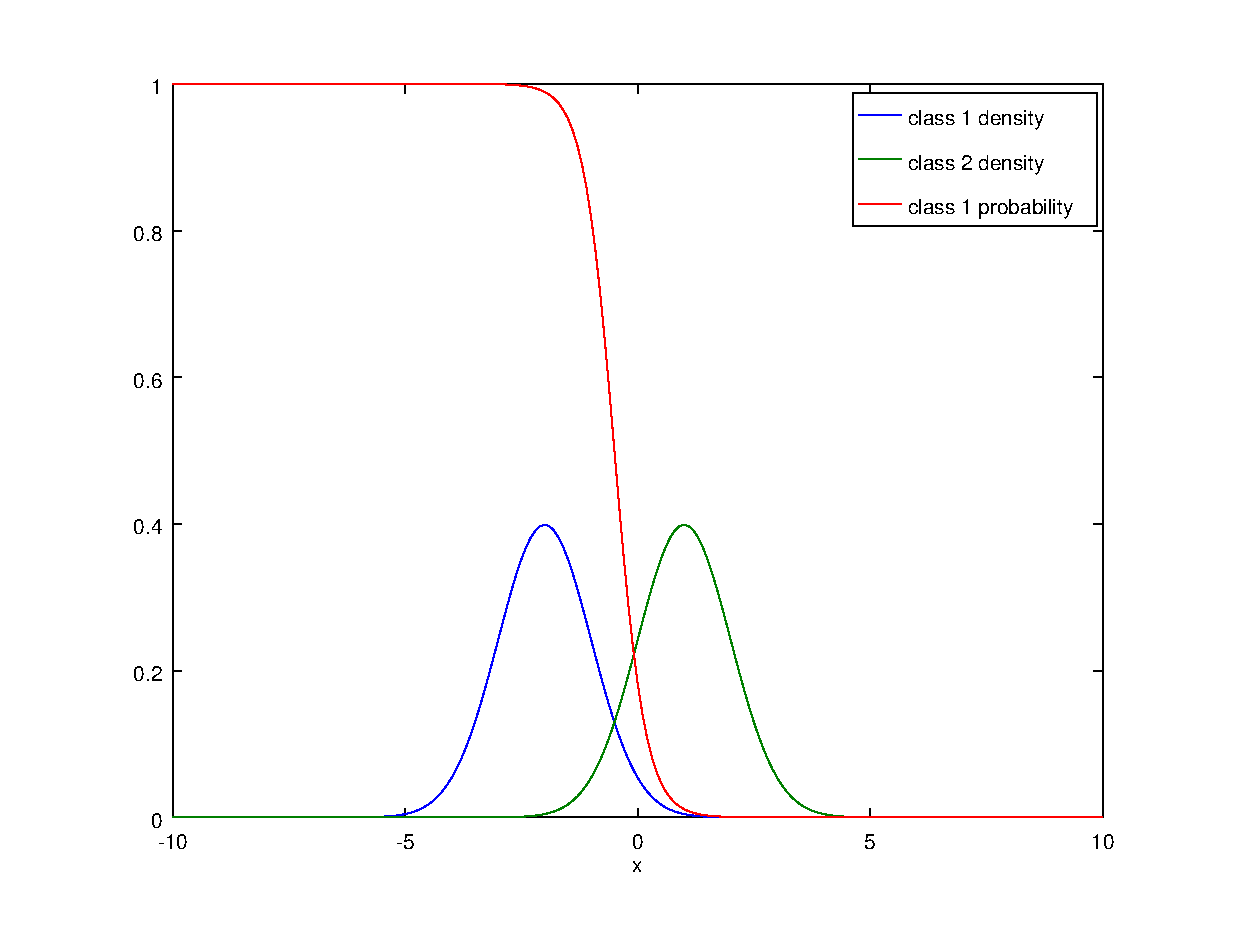
\includegraphics[width=\textwidth]{../figures/equal-variance}
      \caption{Equal prior and variance}
    \end{subfigure}
    \begin{subfigure}{\fwidth}
      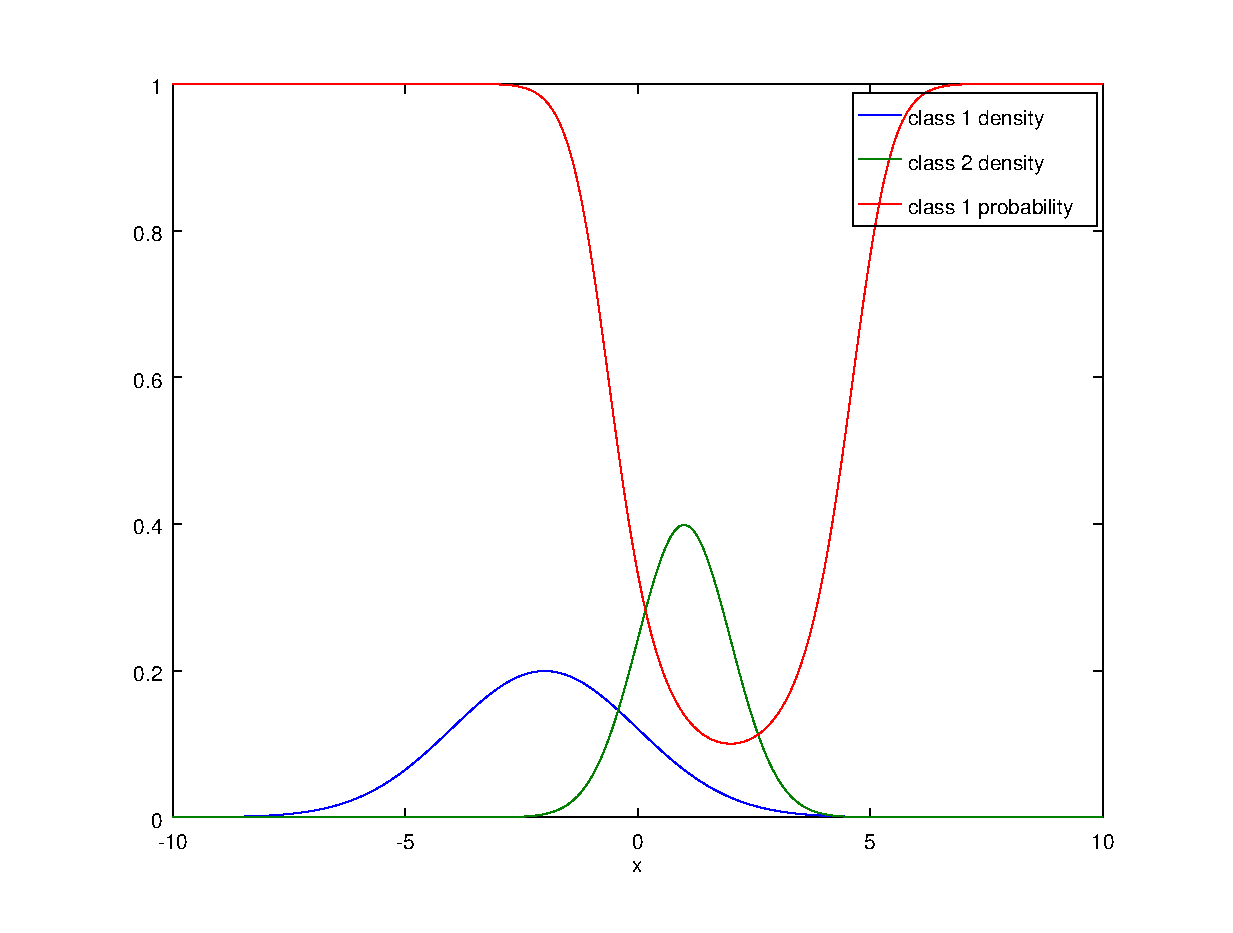
\includegraphics[width=\textwidth]{../figures/unequal-variance}
      \caption{Unequal variance}
    \end{subfigure}
    \begin{subfigure}{\fwidth}
      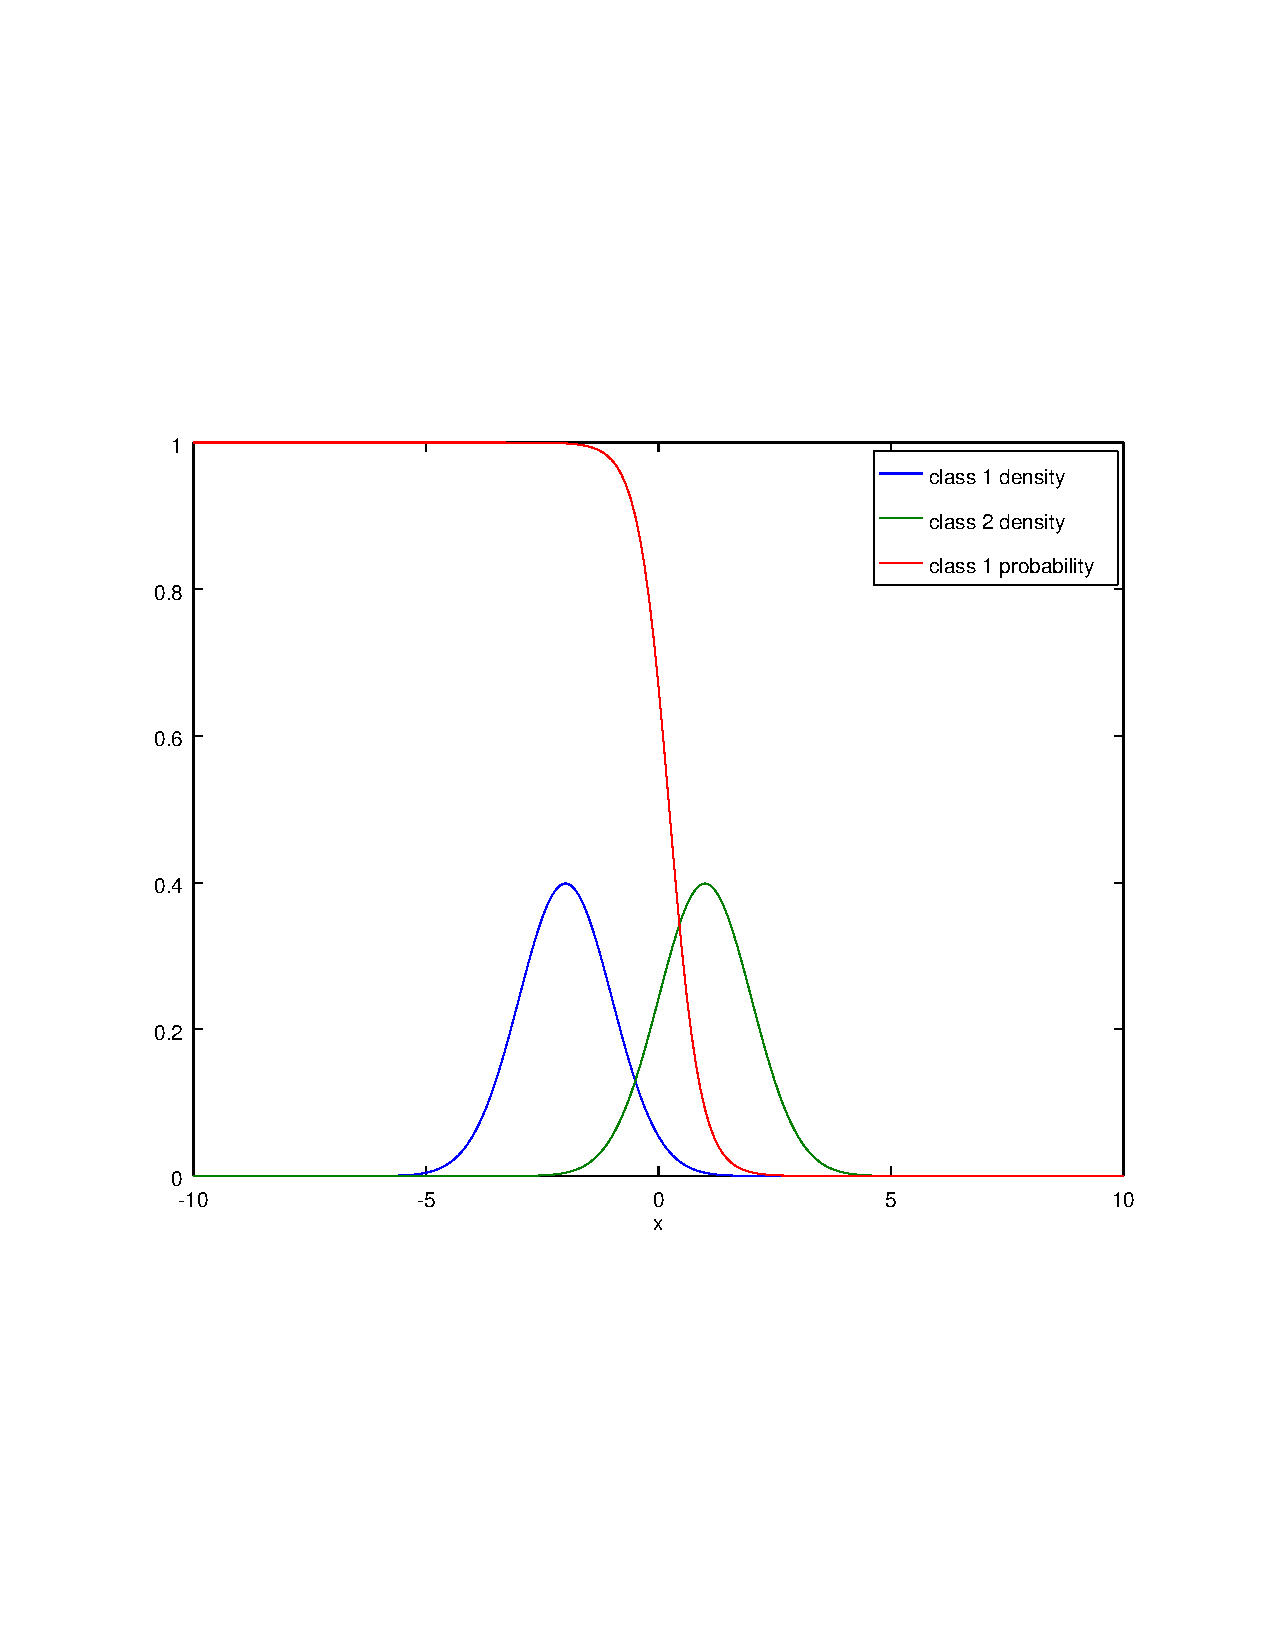
\includegraphics[width=\textwidth]{../figures/unequal-prior}
      \caption{Unequal prior}
    \end{subfigure}
    \caption{The effect of changing variance and prior on the classification decision when we assume a normal distribution.}
    \label{fig:normal-generative}
  \end{figure}
  \begin{example}[Normal distribution]
    A simple example is when $x_t$ is normally distributed in a matter that depends on the class.  Figure~\ref{fig:normal-generative} shows the distribution of $x_t$ for two different classes, with means of $-1$ and $+1$ respectively, for three different case. In the first case, both classes have variance of 1, and we assume the same prior probability for both
    \[
    x_t \mid y_t = 0 \sim \Normal(-1,1),
    \qquad
    x_t \mid y_t = 1 \sim \Normal(1,1)
    \]
    \[
    x_t \mid y_t = 0 \sim \Normal(-1,1),
    \qquad
    x_t \mid y_t = 1 \sim \Normal(1,1)
    \]

  \end{example}
  
  \uncover<5>{
    \alert{But how can we get a probability model in the first place?}
  }
\end{frame}


\begin{frame}
  \frametitle{Subjective probability}
  \only<article>{While probabilities apply to truly random events, they are also useful for representing subjective uncertainty. In this course, we will use a special symbol for subjective probability, $\bel$.}
  \begin{block}{Subjective probability measure $\bel$}
    \begin{itemize}
    \item If we think event $A$ is more likely than $B$, then $\bel(A) > \bel(B)$.
    \item Usual rules of probability apply:
      \begin{enumerate}
      \item $\bel(A) \in [0,1]$.
      \item $\bel(\emptyset) = 0$.
      \item If $A \cap B = \emptyset$, then $\bel(A \cup B) = \bel(A) + \bel(B)$.
      \end{enumerate}
    \end{itemize}
  \end{block}
\end{frame}


\begin{frame}
  \frametitle{Bayesian inference illustration}
  \begin{columns}
    \begin{column}{0.7\textwidth}
      \begin{block}{Use a subjective belief $\bel(\model)$ on $\Model$}
        \begin{itemize}
        \item<1-> \alert{Prior} belief $\bel(\model)$ represents our initial uncertainty.
        \item<2-> We \alert{observe history} $h$.
        \item<3->Each possible $\model$ assigns a \alert{probability} $P_\model(h)$ to $h$.
        \item<4-> We can use this to \alert{update} our belief via Bayes' theorem to obtain the \alert{posterior} belief:
          \[
          \bel(\model \mid h) \propto P_\model(h) \bel(\model)
          \tag{conclusion = evidence $\times$ prior}
          \]
        \end{itemize}
      \end{block}
    \end{column}
    \begin{column}{0.3\textwidth}
      \centering
      \uncover<1->{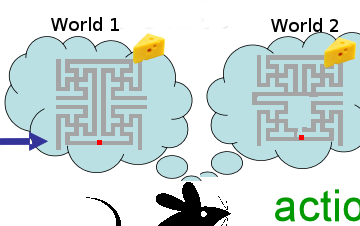
\includegraphics[width=0.5\fwidth]{../figures/rl_worlds}
        \\
        prior
      }
      \\
      \uncover<2->{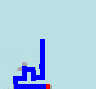
\includegraphics[width=0.5\fwidth]{../figures/rl_observations}
        \\
        evidence
      }
      \\
      \uncover<4->{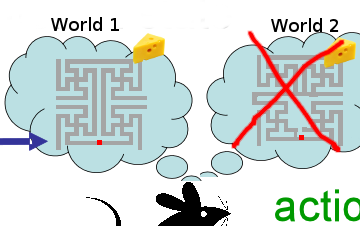
\includegraphics[width=0.5\fwidth]{../figures/rl_worlds2}
        \\ 
        conclusion
      }
    \end{column}
  \end{columns}
\end{frame}




\subsection{Probability and Bayesian inference}
\only<article>{One of the most important methods in machine learning
  and statistics is that of Bayesian inference.  This is the most
  fundamental method of drawing conclusions from data and explicit
  prior assumptions. In Bayesian inference, prior assumptions are
  represented as a probabilities on a space of hypotheses. Each
  hypothesis is seen as a probabilistic model of all possible data
  that we can see.}

\only<article>{Frequently, we want to draw conclusions from data. However, the conclusions are never solely inferred from data, but also depend on prior assumptions about reality.}




\begin{frame}
  \frametitle{Some examples}

  \begin{example}
    John claims to be a medium. He throws a coin $n$ times and predicts its value always correctly. Should we believe that he is a medium?
    \begin{itemize}
    \item $\model_1$: John is a medium.
    \item $\model_0$: John is not a medium.
    \end{itemize}
  \end{example}
  The answer depends on what we \alert{expect} a medium to be able to do, and how likely we thought he'd be a medium in the first place.

  \only<article>{
    \begin{example}
      Traces of DNA are found at a murder scene. We perform a DNA test against a database of $10^4$ citizens registered to be living in the area. We know that the probability of a false positive (that is, the test finding a match by mistake) is $10^{-6}$. If there is a match in the database, does that mean that the citizen was at the scene of the crime?
    \end{example}
  }
\end{frame}





\begin{frame}
  \frametitle{Bayesian inference}
  \only<article>{
    Now let us apply this idea to our specific problem. We already have the probability of the observation for each model, but we just need to define a \emph{prior probability} for each model. Since this is usually completely subjective, we give it another symbol.
  }
  \only<article>{
    \begin{block}{Prior probability}
      The prior probability $\bel$ on a set of models $\Model$ specifies our subjective belief $\bel(\model)$ that each model is true.\footnote{More generally $\bel$ is a probability measure.}
    \end{block}
  }
  \only<article>{
    This allows us to calculate the probability of John being a medium, given the data:
    \[
    \bel(\model_1 \mid \bx) = \frac{\Pr(\bx \mid \model_1) \bel(\model_1)}{\Pr_\bel(\bx)},
    \]
    where
    \[
    \Pr_\bel(\bx) \defn \Pr(\bx \mid \model_1) \bel(\model_1) + \Pr(\bx \mid \model_0) \bel(\model_0).
    \]
    The only thing left to specify is $\bel(\model_1)$, the probability that John is a medium before seeing the data. This is our subjective prior belief that mediums exist and that John is one of them.
    More generally, we can think of Bayesian inference as follows: }
  \begin{itemize}
  \item<1-> \only<article>{We start with a set of } mutually exclusive models $\Model = \{\model_1, \ldots, \model_k\}$.
  \item<2->\only<article>{Each model $\model$ is represented by a specific probabilistic model for any possible data $x$, that is}
    \only<presentation>{Probability model for any data $x$:} $P_\model(x) \equiv \Pr(x \mid \model)$.
  \item<3-> For each model, we have a prior probability $\bel(\model)$ that it is correct.
  \item<4-> \only<article>{After observing the data, we can calculate a posterior probability that the model is correct:}
    \only<presentation>{Posterior probability}
    \[
    \bel(\model \mid x) = \frac{\Pr(x \mid \model) \bel(\model)}{\sum_{\model' \in \Model} \Pr(x \mid \model') \bel(\model')}
    = \frac{P_\model(x) \bel(\model)}{\sum_{\model' \in \Model} P_{\model'} (x) \bel(\model')}.
    \]
  \end{itemize}
  \only<5->{
    \begin{block}{Interpretation}
      \begin{itemize}
      \item $\CM$: Set of all possible models that could describe the data.
      \item $P_\model(x)$: Probability of $x$ under model $\model$.
      \item Alternative notation $\Pr(x \mid \model)$: Probability of $x$ given that model $\model$ is correct.
      \item $\bel(\model)$: Our belief, before seeing the data, that $\model$ is correct.
      \item $\bel(\model \mid x)$: Our belief, aftering seeing the data, that $\model$ is correct.
      \end{itemize}
    \end{block}
    \only<article>{It must be emphasized that $P_\model(x) = \Pr(x \mid \model)$ as they are simply two different notations for the same thing. In words the first can be seen as the probability that model $\model$ assigns to data $x$, while the second as the probability of $x$ if $\model$ is the true model.}
  }
  \only<article>{
    Combining the prior belief with evidence is key in this procedure. Our posterior belief can then be used as a new prior belief when we get more evidence.}
\end{frame}
\begin{frame}
  \begin{exercise}[Continued example for medium]
    \only<article>{ Now let us apply this idea to our specific
      problem. We first make an independence assumption. In particular, we can assume that success and failure comes from a Bernoulli distribution with a parameter depending on the model.}
    \begin{align}
      P_{\model} (x) &= \prod_{t=1}^n P_{\model} (x_t).
                       \tag{independence property}
    \end{align}
    \only<article>{We first need to specify how well a medium could predict. Let's assume that a true medium would be able to predict perfectly, and that a non-medium would only predict randomly. This leads to the following models:}
    \begin{align}
      P_{\model_1}(x_t = 1) &= 1, &P_{\model_1}(x_t = 0) &= 0.
                                                           \tag{true medium model}
      \\
      P_{\model_0}(x_t = 1) &= 1/2, &P_{\model_0}(x_t = 0) &= 1/2.
                                                             \tag{non-medium model}
    \end{align}
    \only<article>{
      The only thing left to specify is $\bel(\model_1)$, the probability
      that John is a medium before seeing the data. This is our
      subjective prior belief that mediums exist and that John is one of
      them.}
    \uncover<3->{
      \begin{align}
        \bel(\model_0) &= 1/2,   &  \bel(\model_1) &= 1/2.
                                                     \tag{prior belief}
      \end{align}
    }
    \only<article>{Combining the prior belief with evidence is key in this
      procedure. Our posterior belief can then be used as a new prior
      belief when we get more evidence.  }
    \uncover<4>{
      \begin{align}
        \bel(\model_1 \mid x) & = \frac{P_{\model_1}(x)
                                \bel(\model_1)}{\Pr_\bel(x)} \tag{posterior belief}
        \\
        \Pr_\bel(x) &\defn P_{\model_1}(x) \bel(\model_1) + P_{\model_0}(x) \bel(\model_0).
                      \tag{marginal distribution}
      \end{align}
    }
    Throw a coin 4 times, and have a classmate make a prediction. What your belief that your classmate is a medium? Is the prior you used reasonable?
  \end{exercise}
\end{frame}


\begin{frame}
  \frametitle{Sequential update of beliefs}
  \only<article>{Assume you have $n$ meteorologists. At each day $t$, each meteorologist $i$ gives a probability $p_{t,\model_i}\defn P_{\model_i}(x_t = \textrm{rain})$ for rain. Consider the case of there being three meteorologists, and each one making the following prediction for the coming week. Start with a uniform prior $\bel(\model) = 1/3$ for each model.}
  {
    \begin{table}[h]
      \begin{tabular}{c|l|l|l|l|l|l|l}
        &M&T&W&T&F&S&S\\
        \hline
        CNN & 0.5 & 0.6 & 0.7 & 0.9 & 0.5 & 0.3 & 0.1\\
        SMHI & 0.3 & 0.7 & 0.8 & 0.9 & 0.5 & 0.2 & 0.1\\
        YR & 0.6 & 0.9 & 0.8 & 0.5 & 0.4 & 0.1 & 0.1\\
        \hline
        Rain? & Y & Y & Y & N & Y & N & N
      \end{tabular}
      \caption{Predictions by three different entities for the probability of rain on a particular day, along with whether or not it actually rained.}
      \label{tab:meteorologists}
    \end{table}
  }
  \begin{exercise}
    \begin{itemize}
    \item $n$ meteorological stations $\cset{\mdp_i}{i=1, \ldots,n}$
    \item The $i$-th station predicts rain $P_{\mdp_i}(x_t \mid x_1, \ldots, x_{t-1})$.
    \item Let $\bel_t(\mdp)$ be our belief at time $t$.
      Derive the next-step belief
      $\bel_{t+1}(\mdp) \defn  \bel_t(\mdp | y_{t})$ in terms of the current belief $\bel_t$.
    \item Write a python function that computes this posterior
    \end{itemize}
  \end{exercise}
  \uncover<2->{
    \[
    \bel_{t+1}(\mdp)
    \defn
    \bel_t(\mdp | x_{t})
    =
    \frac{P_\mdp(x_t \mid x_1, \ldots, x_{t-1}) \bel_t(\mdp)}
    {\sum_{\mdp'} P_{\mdp'}(x_t \mid x_1, \ldots, x_{t-1}) \bel_t(\mdp')}
    \]
  }
\end{frame}



\begin{frame}[label=beta-example]
  \frametitle{Bayesian inference for Bernoulli distributions}
  \only<1>{
    \begin{block}{Estimating a coin's bias}
      A fair coin comes heads $50\%$ of the time. 
      We want to test an unknown coin, which we think may not be completely fair. 
    \end{block}
  }
  \only<1,2>{
    \begin{figure}[h]
      \centering
      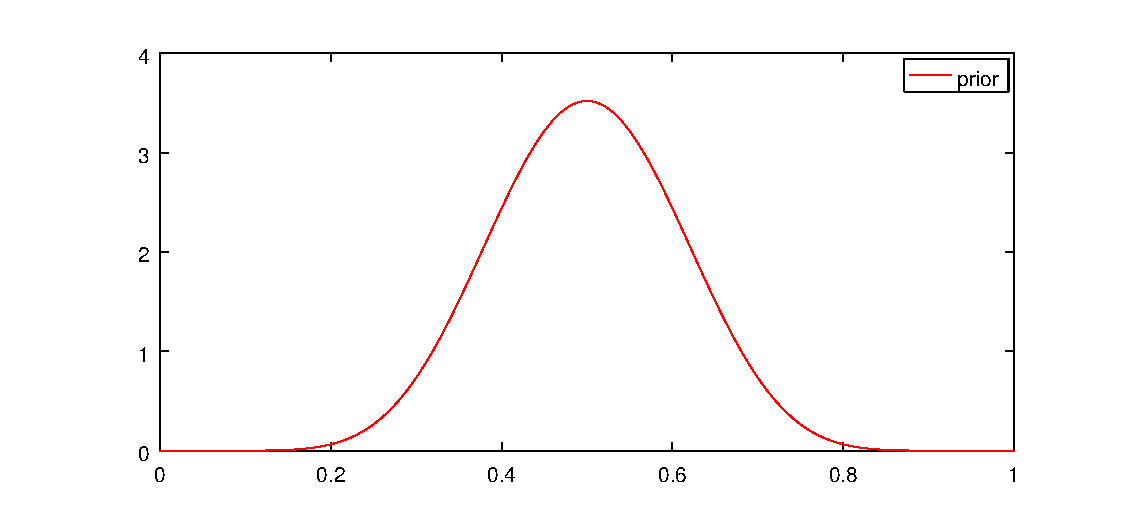
\includegraphics[width=\textwidth]{../figures/beta-prior}
      \caption{Prior belief $\bel$ about the coin bias $\theta$.}
    \end{figure}
  }
  \only<2>{
    For a sequence of throws $x_t \in \{0,1\}$,
    \[
    P_\theta(x) \propto \prod_t \theta^{x_t} (1 - \theta)^{1 - x_t}
    = \theta^{\textrm{\#Heads}} (1 - \theta)^{\textrm{\#Tails}}
    \]
  }
  \only<3>{
    \begin{figure}[h]
      \centering
      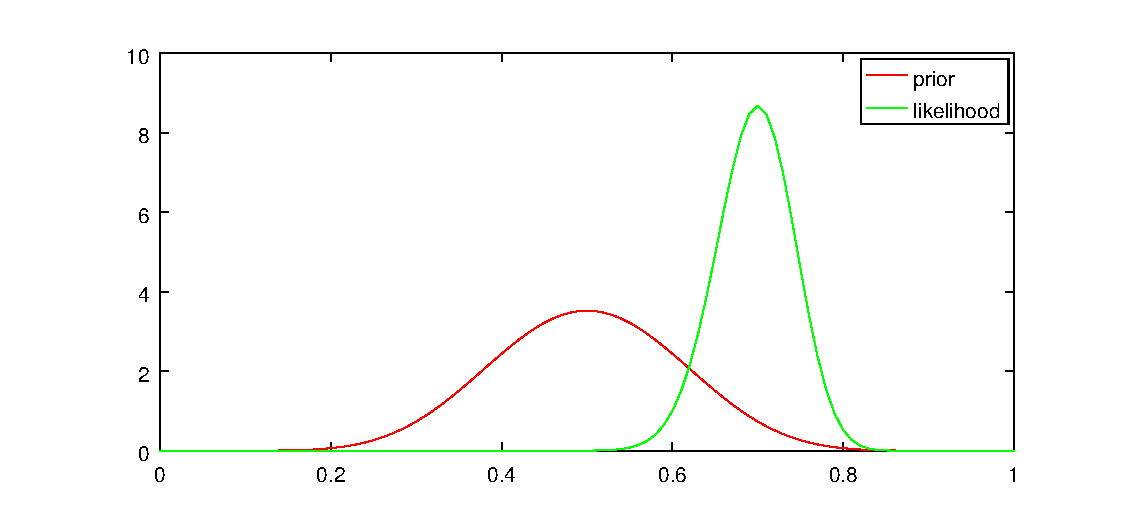
\includegraphics[width=\textwidth]{../figures/beta-likelihood}
      \caption{Prior belief $\bel$ about the coin bias $\theta$ and likelihood of $\theta$ for the data.}
    \end{figure}
    Say we throw the coin 100 times and obtain 70 heads. Then we plot the \alert{likelihood} $P_\theta(x)$ of different models.
  }
  \only<4>{
    \begin{figure}[h]
      \centering
      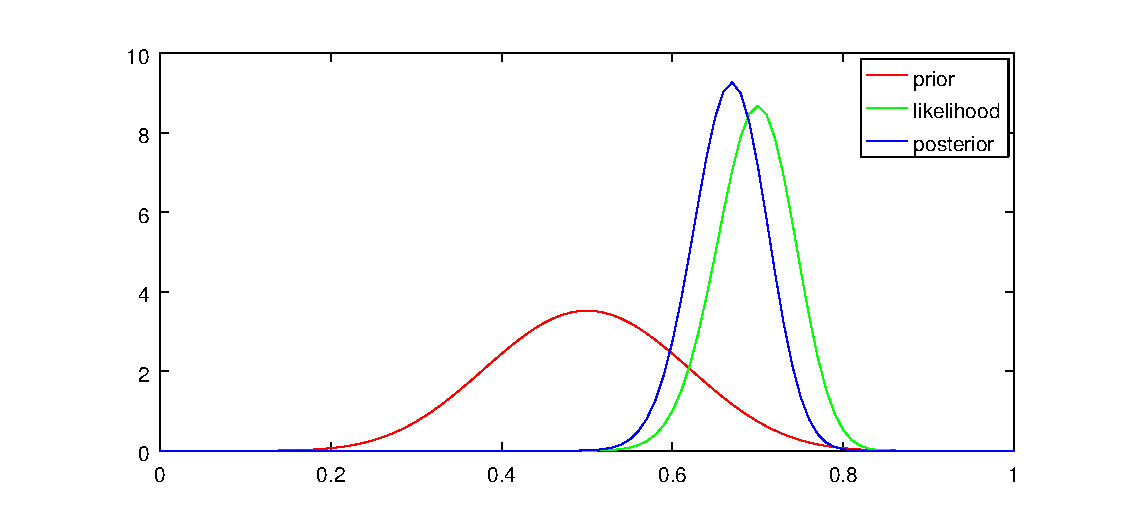
\includegraphics[width=\textwidth]{../figures/beta-posterior}
      \caption{Prior belief $\bel(\theta)$ about the coin bias $\theta$, likelihood of $\theta$ for the data, and posterior belief $\bel(\theta \mid x)$}
    \end{figure}
    From these, we calculate a \alert{posterior} distribution over the correct models. This represents our conclusion given our prior and the data.
  }
  \only<article>{If the prior distribution is described by the so-called Beta density
    \[
    f(\theta \mid \alpha, \beta) \propto \theta^{\alpha -1} (1 - \theta)^{\beta -1}
    \]
    where $\alpha, \beta$ describe the shape of the Beta distribution.
  }
\end{frame}

\subsubsection{Riemann and Lebesgue integrals}
\only<article>{
  Since $\bel$ is a probability measure over models $\Param$, it is always simple to write the posterior probability given some data $x$ in the following terms when $\Param$ is discrete (finite or countable):
  \[
  \bel(\param \mid x) = \frac{P_\param(x) \bel(\param)}{\sum_{\param'} P_{\param'(x) \bel(\param')}.}
  \]
  However, in many situations $\Param$ is uncountable, i.e. $\Param \subset \Reals^k$. Then, as both the prior $\bel$ and the posterior $\bel(\cdot \mid x)$ have to be probability measures on $\Param$, they are defined over subsets of $\Param$. This means that we can write the posterior in terms of Lebesgue integrals:
  \[
  \bel(B \mid x) = \frac{\int_B P_\param(x) \dd \bel(\param)}{\int_\Param P_\param(x) \dd \bel(\param)}.
  \]
  Alternatively, we can abuse notation and use $\bel(\param)$ to describe a density, so that the \emindex{posterior density} is written in terms of a Riemann integral:
  \[
  \bel(\param \mid x) \defn \frac{P_\param(x) \bel(\param) \dd \param}{\int_{\Param} P_{\param'}(x) \bel(\param') \param'}.
  \]
  However, the advantage of the Lebesgue integral notation is that it works the same no matter whether $\Param$ is discrete or continuous.
}
\begin{frame}
  \frametitle{Learning outcomes}
  \begin{block}{Understanding}
    \begin{itemize}
    \item The axioms of probability, marginals and conditional distributions.
    \item The philosophical underpinnings of Bayesianism.
    \item The simple conjugate model for Bernoulli distributions.
    \end{itemize}
  \end{block}
  
  \begin{block}{Skills}
    \begin{itemize}
    \item Be able to calculate with probabilities using the marginal and conditional definitions and Bayes rule.
    \item Being able to implement a simple Bayesian inference algorithm in Python.
    \end{itemize}
  \end{block}

  \begin{block}{Reflection}
    \begin{itemize}
    \item How useful is the Bayesian representation of uncertainty?
    \item How restrictive is the need to select a prior distribution?
    \item Can you think of another way to explicitly represent uncertainty in a way that can incorporate new evidence?
    \end{itemize}
  \end{block}
  
\end{frame}

%%% Local Variables:
%%% mode: latex
%%% TeX-engine: xetex
%%% TeX-master: "notes.tex"
%%% End:
 % Bayesian inference
\section{Hierarchies of decision making problems}
\only<presentation>{
  \begin{frame}
    \tableofcontents[ 
    currentsection, 
    hideothersubsections, 
    sectionstyle=show/shaded
    ] 
  \end{frame}
}


\only<article>{
  All machine learning problems are essentially decision problems. This essentially means replacing some human decisions with machine decisions. One of the simplest decision problems is classification, where you want an algorithm to decide the correct class of some data, but even within this simple framework there is a multitude of decisions to be made. The first is how to frame the classification problem the first place. The second is how to collect, process and annotate the data. The third is choosing the type of classification model to use. The fourth is how to use the collected data to find an optimal classifier within the selected type. After all this has been done, there is the problem of classifying new data. In this course, we will take a holistic view of the problem, and consider each problem in turn, starting from the lowest level and working our way up.}


\subsection{Simple decision problems}
\begin{frame}
  \frametitle{Preferences}
  \only<article>{The simplest decision problem involves selecting one item from a set of choices, such as in the following examples}  
  \begin{example}
    \begin{block}{Food}
      \begin{itemize}
      \item[A] McDonald's cheeseburger
      \item[B] Surstromming
      \item[C] Oatmeal
      \end{itemize}
    \end{block}
    \begin{block}{Money}
      \begin{itemize}
      \item[A] 10,000,000 SEK
      \item[B] 10,000,000 USD
      \item[C] 10,000,000 BTC
      \end{itemize}
    \end{block}
    \begin{block}{Entertainment}
      \begin{itemize}
      \item[A] Ticket to Liseberg
      \item[B] Ticket to Rebstar
      \item[C] Ticket to Nutcracker
      \end{itemize}
    \end{block}
  \end{example}
\end{frame}

\begin{frame}
  \frametitle{Rewards and utilities}
  \only<article>{In the decision theoretic framework, the things we receive are called rewards, and we assign a utility value to each one of them, showing which one we prefer.}
  \begin{itemize}
  \item Each choice is called a \alert{reward} $r \in \CR$.
  \item There is a \alert{utility function} $U : \CR \to \Reals$, assigning values to reward.
  \item We (weakly) prefer $A$ to $B$ iff $U(A) \geq U(B)$.
  \end{itemize}
  \only<article>{In each case, given $U$ the choice between each reward is trivial. We just select the reward:
    \[
      r^* \in \argmax_r U(r)
    \]
    The main difficult is actually selecting the appropriate utility function. In a behavioural context, we simply assume that humans act with respect to a specific utility function. However, figuring out this function from behavioural data is non trivial. ven when this assumption is correct, individuals do not have a common utility function.
  }
  \begin{exercise}
    From your individual preferences, derive a \alert{common utility function} that reflects everybody's preferences in the class for each of the three examples. Is there a simple algorithm for deciding this? Would you consider the outcome fair?
  \end{exercise}
\end{frame}

\begin{frame}
  \frametitle{Preferences among random outcomes}
  \begin{example}
    Would you rather \ldots
    \begin{itemize}
    \item[A] Have 100 EUR now?
    \item[B] Flip a coin, and get 200 EUR if it comes heads?
    \end{itemize}    
  \end{example}
  \uncover<2->{
    \begin{block}{The expected utility hypothesis}
      Rational decision makers prefer choice $A$ to $B$ if
      \[
        \E(U | A) \geq \E(U | B),
      \]
      where the expected utility is
      \[
        \E(U | A) = \sum_r U(r) \Pr(r | A).
      \]
    \end{block}
    In the above example, $r \in \{0, 100, 200\}$ and $U(r)$ is
    increasing, and the coin is fair.
  }
  \begin{itemize}
  \item<3-> If $U$ is convex, we prefer B.
  \item<4-> If $U$ is concave, we prefer A.
  \item<5-> If $U$ is linear, we don't care.
  \end{itemize}
\end{frame}


\begin{frame}
  \frametitle{Uncertain rewards}
  \only<article>{However, in real life, there are many cases where we can only choose between uncertain outcomes. The simplest example are lottery tickets, where rewards are essentially random. However, in many cases the rewards are not really random, but simply uncertain. In those cases it is useful to represent our uncertainty with probabilities as well, even though there is nothing really random.}
  \begin{itemize}
  \item Decisions $\decision \in \Decision$
  \item Each choice is called a \alert{reward} $r \in \CR$.
  \item There is a \alert{utility function} $U : \CR \to \Reals$, assigning values to reward.
  \item We (weakly) prefer $A$ to $B$ iff $U(A) \geq U(B)$.
  \end{itemize}

  \begin{example}
    \begin{columns}
      \begin{column}{0.5\textwidth}
        You are going to work, and it might rain.  What do you do?
        \begin{itemize}
        \item $\decision_1$: Take the umbrella.
        \item $\decision_2$: Risk it!
        \item $\outcome_1$: rain
        \item $\outcome_2$: dry
        \end{itemize}
      \end{column}
      \begin{column}{0.5\textwidth}
        \begin{table}
          \centering
          \begin{tabular}{c|c|c}
            $\Rew(\outcome,\decision)$ & $\decision_1$ & $\decision_2$ \\ %ro: U has only one argument.
            \hline
            $\outcome_1$ & dry, carrying umbrella & wet\\
            $\outcome_2$ & dry, carrying umbrella & dry\\
            \hline
            \hline
            $U[\Rew(\outcome,\decision)]$ & $\decision_1$ & $\decision_2$ \\
            \hline
            $\outcome_1$ & 0 & -10\\
            $\outcome_2$ & 0 & 1
          \end{tabular}
          \caption{Rewards and utilities.}
          \label{tab:rain-utility-function}
        \end{table}

        \begin{itemize}
        \item<2-> $\max_\decision \min_\outcome U = 0$
        \item<3-> $\min_\outcome \max_\decision U = 0$
        \end{itemize}
      \end{column}

    \end{columns}
  \end{example}
\end{frame}



\begin{frame}
  \frametitle{Expected utility}
  \[
    \E (U \mid a) = \sum_r U[\Rew(\outcome, \decision)] \Pr(\outcome \mid \decision)
  \]
  \begin{example}%ro: rather an exercise?
    You are going to work, and it might rain. The forecast said that
    the probability of rain $(\outcome_1)$ was $20\%$. What do you do?
    \begin{itemize}
    \item $\decision_1$: Take the umbrella.
    \item $\decision_2$: Risk it!
    \end{itemize}
    \begin{table}
      \centering
      \begin{tabular}{c|c|c}
        $\Rew(\outcome,\decision)$ & $\decision_1$ & $\decision_2$ \\ %ro: U has only one argument.
        \hline
        $\outcome_1$ & dry, carrying umbrella & wet\\
        $\outcome_2$ & dry, carrying umbrella & dry\\
        \hline
        \hline
        $U[\Rew(\outcome,\decision)]$ & $\decision_1$ & $\decision_2$ \\
        \hline
        $\outcome_1$ & 0 & -10\\
        $\outcome_2$ & 0 & 1\\
        \hline
        \hline
        $\E_P(U \mid \decision)$ & 0 &  -1.2 \\ 
      \end{tabular}
      \caption{Rewards, utilities, expected utility for $20\%$ probability of rain.}
      \label{tab:rain-utility-function}
    \end{table}
  \end{example}
\end{frame}





\subsection{Decision rules}

\only<article>{We now move from simple decisions to decisions that
  depend on some observation. We shall start with a simple problem in applied meteorology. Then we will discuss hypothesis testing as a decision making problem. Finally, we will go through an exercise in Bayesian methods for classification.}

\begin{frame}
  \frametitle{Bayes decision rules}
  Consider the case where outcomes are independent of decisions:
  \[
    \util (P, \decision) \defn \sum_{\model}  \util (\model, \decision) P(\model)
  \]
  This corresponds e.g. to the case where $P(\omega)$ is the belief about an unknown world.
  \begin{definition}[Bayes utility]
    \label{def:bayes-utility}
    The maximising decision for $P$ has an expected utility equal to:
    \begin{equation}
      \BUtil(P) \defn \sup_{\decision \in \Decision} \util (P, \decision).
      \label{eq:bayes-utility}
    \end{equation}
  \end{definition}
\end{frame}




\begin{frame}
  \frametitle{The $n$-meteorologists problem}
  \only<article>{Of course, we may not always just be interested in classification performance in terms of predicting the most likely class. It strongly depends on the problem we are actually wanting to solve. In  biometric authentication, for example, we want to guard against the unlikely event that an impostor will successfully be authenticated. Even if the decision rule that always says 'OK' has the lowest classification error in practice, the expected cost of impostors means that the optimal decision rule must sometimes say 'Failed' even if this leads to false rejections sometimes.}
  \begin{exercise}
    \only<presentation>{
      \only<1>{
        \begin{itemize}
        \item Meteorological models $\CM = \set{\model_1, \ldots, \model_n}$
        \item Rain predictions at time $t$: $p_{t,\model} \defn  P_{\model}(x_t = \textrm{rain})$.
        \item Prior probability $\bel(\model) = 1/n$ for each model.
        \item Should we take the umbrella?
        \end{itemize}
      }
    }
    \only<article>{Assume you have $n$ meteorologists. At each day $t$, each meteorologist $i$ gives a probability $p_{t,\model_i}\defn P_{\model_i}(x_t = \textrm{rain})$ for rain. Consider the case of there being three meteorologists, and each one making the following prediction for the coming week. Start with a uniform prior $\bel(\model) = 1/3$ for each model.}
    {
      \begin{table}[h]
        \begin{tabular}{c|l|l|l|l|l|l|l}
          &M&T&W&T&F&S&S\\
          \hline
          CNN & 0.5 & 0.6 & 0.7 & 0.9 & 0.5 & 0.3 & 0.1\\
          SMHI & 0.3 & 0.7 & 0.8 & 0.9 & 0.5 & 0.2 & 0.1\\
          YR & 0.6 & 0.9 & 0.8 & 0.5 & 0.4 & 0.1 & 0.1\\
          \hline
          Rain? & Y & Y & Y & N & Y & N & N
        \end{tabular}
        \caption{Predictions by three different entities for the probability of rain on a particular day, along with whether or not it actually rained.}
        \label{tab:meteorologists}
      \end{table}
    }
    \uncover<2->{
      \begin{enumerate}
      \item<2-> What is your belief about the quality of each meteorologist after each day? 
      \item<3-> What is your belief about the probability of rain each day? 
        \[
          P_\bel(x_t = \textrm{rain} \mid x_1, x_2, \ldots x_{t-1})
          =
          \sum_{\model \in \Model} P_\model(x_t = \textrm{rain})
          \bel(\model \mid x_1, x_2, \ldots x_{t-1}) 
        \]
      \item<4-> Assume you can decide whether or not to go running each
        day. If you go running and it does not rain, your utility is 1. If
        it rains, it's -10. If you don't go running, your utility is
        0. What is the decision maximising utility in expectation (with respect to the posterior) each
        day?
      \end{enumerate}
    }
  \end{exercise}
\end{frame}


\subsection{Statistical testing}
\only<article>{A common type of decision problem is a statistical test. This arises when we have a set of possible candidate models $\CM$ and we need to be able to decide which model to select after we see the evidence.
  Many times, there is only one model under consideration, $\model_0$, the so-called \alert{null hypothesis}. Then, our only decision is whether or not to accept or reject this hypothesis.}
\begin{frame}
  \frametitle{Simple hypothesis testing}
  \only<article>{Let us start with the simple case of needing to compare two models.}
  \begin{block}{The simple hypothesis test as a decision problem}
    \begin{itemize}
    \item $\CM = \{\model_0, \model_1\}$
    \item $a_0$: Accept model $\model_0$
    \item $a_1$: Accept model $\model_1$
    \end{itemize}
    \begin{table}[H]
      \begin{tabular}{c|cc}
        $\util$& $\model_0$& $\model_1$\\\hline
        $a_0$ & 1 & 0\\
        $a_1$ & 0 & 1
      \end{tabular}
      \caption{Example utility function for simple hypothesis tests.}
    \end{table}
    \only<article>{There is no reason for us to be restricted to this utility function. As it is diagonal, it effectively treats both types of errors in the same way.}
  \end{block}

  \begin{example}[Continuation of the medium example]
    \begin{itemize}
    \item $\model_1$: that John is a medium.
    \item $\model_0$: that John is not a medium.
    \end{itemize}
    \only<article>{
    Let $x_t$ be $0$ if John makes an incorrect prediction at time $t$ and $x_t = 1$ if he makes a correct prediction. Let us once more assume a Bernoulli model, so that John's claim that he can predict our tosses perfectly means that for a sequence of tosses $\bx = x_1, \ldots, x_n$,
    \[
      P_{\model_1}(\bx) = \begin{cases}
        1, & x_t = 1 \forall t \in [n]\\
        0, & \exists t \in [n] : x_t = 0.
      \end{cases}
    \]
    That is, the probability of perfectly correct predictions is 1, and that of one or more incorrect prediction is 0. For the other model, we can assume that all draws are independently and identically distributed from a fair coin. Consequently, no matter what John's predictions are, we have that:
    \[
      P_{\model_0}(\bx = 1 \ldots 1) = 2^{-n}.
    \]
    So, for the given example, as stated, we have the following facts:
    \begin{itemize}
    \item If John makes one or more mistakes, then $\Pr(\bx \mid \model_1) = 0$ and $\Pr(\bx \mid \model_0) = 2^{-n}$. Thus, we should perhaps say that then John is not a medium
    \item If John makes no mistakes at all, then 
      \begin{align}
        \Pr(\bx = 1, \ldots, 1 \mid \model_1) &= 1,
        &
          \Pr(\bx = 1, \ldots, 1 \mid \model_0) &= 2^{-n}.
      \end{align}
    \end{itemize}
    Now we can calculate the posterior distribution, which is
    \[
      \bel(\model_1 \mid \bx = 1, \ldots, 1) = \frac{1 \times \bel(\model_1)}{1 \times \bel(model_1) + 2^{-n} (1 - \bel(\model_1))}.
    \]
    Our expected utility for taking action $a_0$ is actually
  }
  \[
    \E_\bel(\util \mid a_0) = 1 \times \bel(\model_0 \mid \bx) + 0 \times \bel(\model_1 \mid \bx), \qquad
    \E_\bel(\util \mid a_1) = 0 \times \bel(\model_0 \mid \bx) + 1 \times \bel(\model_1 \mid \bx)
  \]
  \end{example}
  
\end{frame}


\begin{frame}
  \frametitle{Null hypothesis test}
  Many times, there is only one model under consideration, $\model_0$, the so-called \alert{null hypothesis}. \only<article>{ This happens when, for example, we have no simple way of defining an appropriate alternative. Consider the example of the medium: How should we expect a medium to predict? Then, our only decision is whether or not to accept or reject this hypothesis.}
  \begin{block}{The null hypothesis test as a decision problem}
    \begin{itemize}
    \item $a_0$: Accept model $\model_0$
    \item $a_1$: Reject model $\model_0$
    \end{itemize}
  \end{block}

  \begin{example}{Construction of the test for the medium}
  \begin{itemize}
  \item<2-> $\model_0$ is simply the $\Bernoulli(1/2)$ model: responses are by chance.
  \item<3-> We need to design a policy $\pol(a \mid \bx)$ that accepts or rejects depending on the data.
  \item<4-> Since there is no alternative model, we can only construct this policy according to its properties when $\model_0$ is true.
  \item<5-> In particular, we can fix a policy that only chooses $a_1$ when $\model_0$ is true a proportion $\delta$ of the time.
  \item<6-> This can be done by construcing a threshold test from the inverse-CDF.
  \end{itemize}
\end{example}
\end{frame}
\begin{frame}
  \frametitle{Using $p$-values to construct statistical tests}
  \begin{definition}[Null statistical test]
    \only<article>{
      A statistical test $\pol$ is a decision rule for accepting or rejecting a hypothesis on the basis of evidence. A $p$-value test rejects a hypothesis whenever the value of the statistic $f(x)$ is smaller than a threshold.}
      The statistic $f : \CX \to [0,1]$ is  designed to have the property:
  \[
    P_{\model_0}(\cset{x}{f(x) \leq \delta}) = \delta.
  \]
  If our decision rule is:
  \[
    \pol(a \mid x) =
    \begin{cases}
      a_0, & f(x) \leq \delta\\
      a_1, & f(x) > \delta,
    \end{cases}
  \]
  the probability of rejecting the null hypothesis when it is true is exactly $\delta$.
\end{definition}
\only<presentation>{The value of the statistic $f(x)$, otherwise known as the \alert{$p$-value}, is uninformative.}
\only<article>{This is because, by definition, $f(x)$ has a uniform distribution under $\model_0$. Hence the value of $f(x)$ itself is uninformative: high and low values are equally likely. In theory we should simply choose $\delta$ before seeing the data and just accept or reject based on whether $f(x) \leq \delta$. However nobody does that in practice, meaning that $p$-values are used incorrectly. Better not to use them at all, if uncertain about their meaning.}
\end{frame}
\begin{frame}
  \frametitle{Issues with $p$-values}
  \begin{itemize}
  \item They only measure quality of fit \alert{on the data}.
  \item Not robust to model misspecification. \only<article>{For example, zero-mean testing using the $\chi^2$-test has a normality assumption.}
  \item They ignore effect sizes. \only<article>{For example, a linear analysis may determine that there is a significant deviation from zero-mean, but with only a small effect size of 0.01. Thus, reporting only the $p$-value is misleading}
  \item They do not consider prior information. 
  \item They do not represent the probability of having made an error. \only<article>{In particular, a $p$-value of $\delta$ does not mean that the probability that the null hypothesis is false given the data $x$, is $\delta$, i.e. $\delta \neq \Pr(\neg \model_0 \mid x)$.}
  \item The null-rejection error probability is the same irrespective of the amount of data.
  \end{itemize}
\end{frame}

\begin{frame}\frametitle{$p$-values for the medium example}
  \only<article>{Let us consider the example of the medium.}
  \begin{itemize}
  \item<2->$\model_0$ is simply the $\Bernoulli(1/2)$ model:
    responses are by chance. 
  \item<3->CDF: $P_{\model_0}(N \leq n \mid K = 100)$ \only<article> {is the probability of at most $N$ successes if we throw the coin 100 times. This is in fact the cumulative probability function of the binomial distribution. Recall that the binomial represents the distribution for the number of successes of independent experiments, each following a Bernoulli distribution.}
  \item<4->ICDF:  the number of successes that will happen with probability at least $\delta$
  \item<5->e.g. we'll get at most 50 successes a proportion $\delta = 1/2$ of the time.
  \item<6>Using the (inverse) CDF we can construct a policy $\pol$ that selects $a_1$ when $\model_0$ is true only a $\delta$ portion of the time, for any choice of $\delta$.
  \end{itemize}
  \begin{columns}
    \setlength\fheight{0.33\columnwidth}
    \setlength\fwidth{0.33\columnwidth}
    \begin{column}{0.5\textwidth}
      \only<3,4,5,6>{% This file was created by matlab2tikz.
%
%The latest updates can be retrieved from
%  http://www.mathworks.com/matlabcentral/fileexchange/22022-matlab2tikz-matlab2tikz
%where you can also make suggestions and rate matlab2tikz.
%
\begin{tikzpicture}

\begin{axis}[%
width=\fwidth,
height=0.831\fheight,
at={(0\fwidth,0\fheight)},
scale only axis,
xmin=0,
xmax=100,
xlabel={Number of successes},
ymin=0,
ymax=1,
ylabel={Probability of less than N successes},
axis background/.style={fill=white}
]
\addplot [color=blue, forget plot]
  table[row sep=crcr]{%
0	7.8886090522101e-31\\
1	7.96749514273217e-29\\
2	3.98453643227134e-27\\
3	1.31543344806511e-25\\
4	3.2248444478818e-24\\
5	6.26162256269277e-23\\
6	1.0029797609618e-21\\
7	1.36307186640302e-20\\
8	1.60428183412199e-19\\
9	1.66102448972682e-18\\
10	1.53164508771899e-17\\
11	1.27042666774617e-16\\
12	9.5567876801385e-16\\
13	6.56490776101789e-15\\
14	4.14222593604009e-14\\
15	2.41271075196861e-13\\
16	1.30296790932804e-12\\
17	6.54899932503508e-12\\
18	3.07390330752401e-11\\
19	1.35138126102441e-10\\
20	5.57954452862595e-10\\
21	2.1686833167108e-09\\
22	7.9526642368932e-09\\
23	2.75679038792502e-08\\
24	9.05001310651458e-08\\
25	2.81814101710274e-07\\
26	8.33681324725063e-07\\
27	2.34620630632112e-06\\
28	6.28957500833936e-06\\
29	1.60800076478334e-05\\
30	3.92506982279687e-05\\
31	9.15716124411769e-05\\
32	0.000204388583713412\\
33	0.000436859918456193\\
34	0.000894965195743431\\
35	0.00175882086148508\\
36	0.00331856025796311\\
37	0.00601648786268185\\
38	0.0104893678389258\\
39	0.0176001001088524\\
40	0.0284439668204906\\
41	0.044313040057034\\
42	0.0666053096036057\\
43	0.0966739522478211\\
44	0.135626512036918\\
45	0.184100808663348\\
46	0.242059206803646\\
47	0.308649706794632\\
48	0.382176717201337\\
49	0.460205381306407\\
50	0.539794618693593\\
51	0.617823282798662\\
52	0.691350293205368\\
53	0.757940793196354\\
54	0.815899191336652\\
55	0.864373487963082\\
56	0.903326047752179\\
57	0.933394690396394\\
58	0.955686959942966\\
59	0.971556033179509\\
60	0.982399899891148\\
61	0.989510632161074\\
62	0.993983512137318\\
63	0.996681439742037\\
64	0.998241179138515\\
65	0.999105034804257\\
66	0.999563140081544\\
67	0.999795611416287\\
68	0.999908428387559\\
69	0.999960749301772\\
70	0.999983919992352\\
71	0.999993710424992\\
72	0.999997653793694\\
73	0.999999166318675\\
74	0.999999718185898\\
75	0.999999909499869\\
76	0.999999972432096\\
77	0.999999992047336\\
78	0.999999997831317\\
79	0.999999999442046\\
80	0.999999999864862\\
81	0.999999999969261\\
82	0.999999999993451\\
83	0.999999999998697\\
84	0.999999999999759\\
85	0.999999999999959\\
86	0.999999999999993\\
87	0.999999999999999\\
88	1\\
89	1\\
90	1\\
91	1\\
92	1\\
93	1\\
94	1\\
95	1\\
96	1\\
97	1\\
98	1\\
99	1\\
100	1\\
};
\end{axis}
\end{tikzpicture}%}      
    \end{column}
    \begin{column}{0.5\textwidth}
      \only<4,5,6>{% This file was created by matlab2tikz.
%
%The latest updates can be retrieved from
%  http://www.mathworks.com/matlabcentral/fileexchange/22022-matlab2tikz-matlab2tikz
%where you can also make suggestions and rate matlab2tikz.
%
\begin{tikzpicture}

\begin{axis}[%
width=\fwidth,
height=0.831\fheight,
at={(0\fwidth,0\fheight)},
scale only axis,
xmin=0,
xmax=1,
xlabel={Probability of less than N successes},
ymin=0,
ymax=100,
ylabel={Number of successes},
axis background/.style={fill=white}
]
\addplot [color=blue, forget plot]
  table[row sep=crcr]{%
0	0\\
0.01	38\\
0.02	40\\
0.03	41\\
0.04	41\\
0.05	42\\
0.06	42\\
0.07	43\\
0.08	43\\
0.09	43\\
0.1	44\\
0.11	44\\
0.12	44\\
0.13	44\\
0.14	45\\
0.15	45\\
0.16	45\\
0.17	45\\
0.18	45\\
0.19	46\\
0.2	46\\
0.21	46\\
0.22	46\\
0.23	46\\
0.24	46\\
0.25	47\\
0.26	47\\
0.27	47\\
0.28	47\\
0.29	47\\
0.3	47\\
0.31	48\\
0.32	48\\
0.33	48\\
0.34	48\\
0.35	48\\
0.36	48\\
0.37	48\\
0.38	48\\
0.39	49\\
0.4	49\\
0.41	49\\
0.42	49\\
0.43	49\\
0.44	49\\
0.45	49\\
0.46	49\\
0.47	50\\
0.48	50\\
0.49	50\\
0.5	50\\
0.51	50\\
0.52	50\\
0.53	50\\
0.54	51\\
0.55	51\\
0.56	51\\
0.57	51\\
0.58	51\\
0.59	51\\
0.6	51\\
0.61	51\\
0.62	52\\
0.63	52\\
0.64	52\\
0.65	52\\
0.66	52\\
0.67	52\\
0.68	52\\
0.69	52\\
0.7	53\\
0.71	53\\
0.72	53\\
0.73	53\\
0.74	53\\
0.75	53\\
0.76	54\\
0.77	54\\
0.78	54\\
0.79	54\\
0.8	54\\
0.81	54\\
0.82	55\\
0.83	55\\
0.84	55\\
0.85	55\\
0.86	55\\
0.87	56\\
0.88	56\\
0.89	56\\
0.9	56\\
0.91	57\\
0.92	57\\
0.93	57\\
0.94	58\\
0.95	58\\
0.96	59\\
0.97	59\\
0.98	60\\
0.99	62\\
1	86\\
};
\end{axis}
\end{tikzpicture}%}
    \end{column}
  \end{columns}    
\end{frame}



\begin{frame}
  \frametitle{Building a test}
  \begin{block}{The test statistic}
    We want the test to reflect that we don't have a significant number of failures.
    \[
    f(x) = 1 - \textrm{binocdf}(\sum_{t=1}^n x_t, n, 0.5)
    \]
  \end{block}
  \begin{alertblock}{What $f(x)$ is and is not}
    \begin{itemize}
    \item It is a \textbf{statistic} which is $\leq \delta$ a $\delta$ portion of the time when $\model_0$ is true.
    \item It is \textbf{not} the probability of observing $x$ under $\model_0$.
    \item It is \textbf{not} the probability of $\model_0$ given $x$.
    \end{itemize}
  \end{alertblock}
\end{frame}
\begin{frame}
  \begin{exercise}
    \begin{itemize}
    \item<1-> Let us throw a coin 8 times.
    \item<2-> Select a $p$-value threshold so that $\delta = 0.05$. 
      For 8 throws, this corresponds to \uncover<3->{$ > 6$ successes.}
    \item<3-> Let's calculate the $p$-value for each one of you
    \end{itemize}
    \only<2,3>{
      % This file was created by matlab2tikz.
%
%The latest updates can be retrieved from
%  http://www.mathworks.com/matlabcentral/fileexchange/22022-matlab2tikz-matlab2tikz
%where you can also make suggestions and rate matlab2tikz.
%
\begin{tikzpicture}

\begin{axis}[%
width=0.951\fwidth,
height=\fheight,
at={(0\fwidth,0\fheight)},
scale only axis,
xmode=log,
xmin=1,
xmax=1000,
xminorticks=true,
xlabel={Amount of throws},
ymin=0.5,
ymax=1,
ylabel={Success rate},
axis background/.style={fill=white},
title={The rejection threshold as data increases}
]
\addplot [color=blue, forget plot]
  table[row sep=crcr]{%
1	1\\
2	1\\
3	1\\
4	1\\
5	0.8\\
6	0.833333333333333\\
7	0.857142857142857\\
8	0.75\\
9	0.777777777777778\\
10	0.8\\
11	0.727272727272727\\
12	0.75\\
13	0.692307692307692\\
14	0.714285714285714\\
15	0.733333333333333\\
16	0.6875\\
17	0.705882352941177\\
18	0.666666666666667\\
19	0.684210526315789\\
20	0.7\\
21	0.666666666666667\\
22	0.681818181818182\\
23	0.652173913043478\\
24	0.666666666666667\\
25	0.68\\
26	0.653846153846154\\
27	0.666666666666667\\
28	0.642857142857143\\
29	0.655172413793103\\
30	0.633333333333333\\
31	0.645161290322581\\
32	0.65625\\
33	0.636363636363636\\
34	0.647058823529412\\
35	0.628571428571429\\
36	0.638888888888889\\
37	0.621621621621622\\
38	0.631578947368421\\
39	0.641025641025641\\
40	0.625\\
41	0.634146341463415\\
42	0.619047619047619\\
43	0.627906976744186\\
44	0.613636363636364\\
45	0.622222222222222\\
46	0.630434782608696\\
47	0.617021276595745\\
48	0.625\\
49	0.612244897959184\\
50	0.62\\
51	0.607843137254902\\
52	0.615384615384615\\
53	0.60377358490566\\
54	0.611111111111111\\
55	0.618181818181818\\
56	0.607142857142857\\
57	0.614035087719298\\
58	0.603448275862069\\
59	0.610169491525424\\
60	0.6\\
61	0.60655737704918\\
62	0.596774193548387\\
63	0.603174603174603\\
64	0.609375\\
65	0.6\\
66	0.606060606060606\\
67	0.597014925373134\\
68	0.602941176470588\\
69	0.594202898550725\\
70	0.6\\
71	0.591549295774648\\
72	0.597222222222222\\
73	0.602739726027397\\
74	0.594594594594595\\
75	0.6\\
76	0.592105263157895\\
77	0.597402597402597\\
78	0.58974358974359\\
79	0.594936708860759\\
80	0.5875\\
81	0.592592592592593\\
82	0.585365853658537\\
83	0.590361445783133\\
84	0.595238095238095\\
85	0.588235294117647\\
86	0.593023255813954\\
87	0.586206896551724\\
88	0.590909090909091\\
89	0.584269662921348\\
90	0.588888888888889\\
91	0.582417582417582\\
92	0.58695652173913\\
93	0.580645161290323\\
94	0.585106382978723\\
95	0.589473684210526\\
96	0.583333333333333\\
97	0.587628865979381\\
98	0.581632653061224\\
99	0.585858585858586\\
100	0.58\\
101	0.584158415841584\\
102	0.57843137254902\\
103	0.58252427184466\\
104	0.576923076923077\\
105	0.580952380952381\\
106	0.575471698113208\\
107	0.579439252336449\\
108	0.583333333333333\\
109	0.577981651376147\\
110	0.581818181818182\\
111	0.576576576576577\\
112	0.580357142857143\\
113	0.575221238938053\\
114	0.578947368421053\\
115	0.573913043478261\\
116	0.577586206896552\\
117	0.572649572649573\\
118	0.576271186440678\\
119	0.571428571428571\\
120	0.575\\
121	0.578512396694215\\
122	0.573770491803279\\
123	0.577235772357724\\
124	0.57258064516129\\
125	0.576\\
126	0.571428571428571\\
127	0.574803149606299\\
128	0.5703125\\
129	0.573643410852713\\
130	0.569230769230769\\
131	0.572519083969466\\
132	0.568181818181818\\
133	0.571428571428571\\
134	0.574626865671642\\
135	0.57037037037037\\
136	0.573529411764706\\
137	0.569343065693431\\
138	0.572463768115942\\
139	0.568345323741007\\
140	0.571428571428571\\
141	0.567375886524823\\
142	0.570422535211268\\
143	0.566433566433566\\
144	0.569444444444444\\
145	0.56551724137931\\
146	0.568493150684932\\
147	0.564625850340136\\
148	0.567567567567568\\
149	0.570469798657718\\
150	0.566666666666667\\
151	0.56953642384106\\
152	0.565789473684211\\
153	0.568627450980392\\
154	0.564935064935065\\
155	0.567741935483871\\
156	0.564102564102564\\
157	0.56687898089172\\
158	0.563291139240506\\
159	0.566037735849057\\
160	0.5625\\
161	0.565217391304348\\
162	0.561728395061728\\
163	0.56441717791411\\
164	0.567073170731707\\
165	0.563636363636364\\
166	0.566265060240964\\
167	0.562874251497006\\
168	0.56547619047619\\
169	0.562130177514793\\
170	0.564705882352941\\
171	0.56140350877193\\
172	0.563953488372093\\
173	0.560693641618497\\
174	0.563218390804598\\
175	0.56\\
176	0.5625\\
177	0.559322033898305\\
178	0.561797752808989\\
179	0.558659217877095\\
180	0.561111111111111\\
181	0.56353591160221\\
182	0.56043956043956\\
183	0.562841530054645\\
184	0.559782608695652\\
185	0.562162162162162\\
186	0.559139784946237\\
187	0.561497326203209\\
188	0.558510638297872\\
189	0.560846560846561\\
190	0.557894736842105\\
191	0.56020942408377\\
192	0.557291666666667\\
193	0.559585492227979\\
194	0.556701030927835\\
195	0.558974358974359\\
196	0.561224489795918\\
197	0.558375634517767\\
198	0.560606060606061\\
199	0.557788944723618\\
200	0.56\\
201	0.557213930348259\\
202	0.559405940594059\\
203	0.556650246305419\\
204	0.558823529411765\\
205	0.55609756097561\\
206	0.558252427184466\\
207	0.555555555555556\\
208	0.557692307692308\\
209	0.555023923444976\\
210	0.557142857142857\\
211	0.554502369668246\\
212	0.556603773584906\\
213	0.553990610328638\\
214	0.55607476635514\\
215	0.558139534883721\\
216	0.555555555555556\\
217	0.557603686635945\\
218	0.555045871559633\\
219	0.557077625570776\\
220	0.554545454545455\\
221	0.556561085972851\\
222	0.554054054054054\\
223	0.556053811659193\\
224	0.553571428571429\\
225	0.555555555555556\\
226	0.553097345132743\\
227	0.555066079295154\\
228	0.552631578947368\\
229	0.554585152838428\\
230	0.552173913043478\\
231	0.554112554112554\\
232	0.556034482758621\\
233	0.553648068669528\\
234	0.555555555555556\\
235	0.553191489361702\\
236	0.555084745762712\\
237	0.552742616033755\\
238	0.554621848739496\\
239	0.552301255230126\\
240	0.554166666666667\\
241	0.551867219917012\\
242	0.553719008264463\\
243	0.551440329218107\\
244	0.55327868852459\\
245	0.551020408163265\\
246	0.552845528455285\\
247	0.550607287449393\\
248	0.55241935483871\\
249	0.550200803212851\\
250	0.552\\
251	0.553784860557769\\
252	0.551587301587302\\
253	0.553359683794466\\
254	0.551181102362205\\
255	0.552941176470588\\
256	0.55078125\\
257	0.552529182879377\\
258	0.550387596899225\\
259	0.552123552123552\\
260	0.55\\
261	0.551724137931034\\
262	0.549618320610687\\
263	0.551330798479088\\
264	0.549242424242424\\
265	0.550943396226415\\
266	0.548872180451128\\
267	0.550561797752809\\
268	0.548507462686567\\
269	0.550185873605948\\
270	0.551851851851852\\
271	0.549815498154982\\
272	0.551470588235294\\
273	0.549450549450549\\
274	0.551094890510949\\
275	0.549090909090909\\
276	0.550724637681159\\
277	0.548736462093863\\
278	0.550359712230216\\
279	0.548387096774194\\
280	0.55\\
281	0.548042704626335\\
282	0.549645390070922\\
283	0.547703180212014\\
284	0.549295774647887\\
285	0.547368421052632\\
286	0.548951048951049\\
287	0.547038327526132\\
288	0.548611111111111\\
289	0.546712802768166\\
290	0.548275862068966\\
291	0.549828178694158\\
292	0.547945205479452\\
293	0.549488054607508\\
294	0.547619047619048\\
295	0.549152542372881\\
296	0.547297297297297\\
297	0.548821548821549\\
298	0.546979865771812\\
299	0.548494983277592\\
300	0.546666666666667\\
301	0.548172757475083\\
302	0.54635761589404\\
303	0.547854785478548\\
304	0.546052631578947\\
305	0.547540983606557\\
306	0.545751633986928\\
307	0.547231270358306\\
308	0.545454545454545\\
309	0.546925566343042\\
310	0.545161290322581\\
311	0.546623794212219\\
312	0.548076923076923\\
313	0.546325878594249\\
314	0.547770700636943\\
315	0.546031746031746\\
316	0.54746835443038\\
317	0.545741324921136\\
318	0.547169811320755\\
319	0.545454545454545\\
320	0.546875\\
321	0.545171339563863\\
322	0.546583850931677\\
323	0.544891640866873\\
324	0.546296296296296\\
325	0.544615384615385\\
326	0.54601226993865\\
327	0.54434250764526\\
328	0.545731707317073\\
329	0.544072948328267\\
330	0.545454545454545\\
331	0.54380664652568\\
332	0.545180722891566\\
333	0.546546546546547\\
334	0.544910179640719\\
335	0.546268656716418\\
336	0.544642857142857\\
337	0.545994065281899\\
338	0.544378698224852\\
339	0.545722713864307\\
340	0.544117647058823\\
341	0.545454545454545\\
342	0.543859649122807\\
343	0.545189504373178\\
344	0.543604651162791\\
345	0.544927536231884\\
346	0.543352601156069\\
347	0.544668587896254\\
348	0.543103448275862\\
349	0.544412607449857\\
350	0.542857142857143\\
351	0.544159544159544\\
352	0.542613636363636\\
353	0.543909348441926\\
354	0.542372881355932\\
355	0.543661971830986\\
356	0.544943820224719\\
357	0.543417366946779\\
358	0.544692737430168\\
359	0.543175487465181\\
360	0.544444444444444\\
361	0.542936288088643\\
362	0.544198895027624\\
363	0.542699724517906\\
364	0.543956043956044\\
365	0.542465753424658\\
366	0.543715846994536\\
367	0.542234332425068\\
368	0.543478260869565\\
369	0.5420054200542\\
370	0.543243243243243\\
371	0.54177897574124\\
372	0.543010752688172\\
373	0.541554959785523\\
374	0.542780748663102\\
375	0.541333333333333\\
376	0.542553191489362\\
377	0.541114058355438\\
378	0.542328042328042\\
379	0.54353562005277\\
380	0.542105263157895\\
381	0.543307086614173\\
382	0.541884816753927\\
383	0.543080939947781\\
384	0.541666666666667\\
385	0.542857142857143\\
386	0.541450777202073\\
387	0.542635658914729\\
388	0.541237113402062\\
389	0.542416452442159\\
390	0.541025641025641\\
391	0.542199488491049\\
392	0.540816326530612\\
393	0.541984732824427\\
394	0.540609137055838\\
395	0.541772151898734\\
396	0.54040404040404\\
397	0.541561712846348\\
398	0.540201005025126\\
399	0.541353383458647\\
400	0.54\\
401	0.541147132169576\\
402	0.539800995024876\\
403	0.540942928039702\\
404	0.542079207920792\\
405	0.540740740740741\\
406	0.541871921182266\\
407	0.540540540540541\\
408	0.541666666666667\\
409	0.540342298288509\\
410	0.541463414634146\\
411	0.54014598540146\\
412	0.54126213592233\\
413	0.539951573849879\\
414	0.541062801932367\\
415	0.539759036144578\\
416	0.540865384615385\\
417	0.539568345323741\\
418	0.54066985645933\\
419	0.539379474940334\\
420	0.54047619047619\\
421	0.539192399049881\\
422	0.540284360189573\\
423	0.539007092198582\\
424	0.540094339622642\\
425	0.538823529411765\\
426	0.539906103286385\\
427	0.53864168618267\\
428	0.539719626168224\\
429	0.540792540792541\\
430	0.53953488372093\\
431	0.540603248259861\\
432	0.539351851851852\\
433	0.540415704387991\\
434	0.539170506912442\\
435	0.540229885057471\\
436	0.538990825688073\\
437	0.540045766590389\\
438	0.538812785388128\\
439	0.539863325740319\\
440	0.538636363636364\\
441	0.53968253968254\\
442	0.538461538461538\\
443	0.539503386004515\\
444	0.538288288288288\\
445	0.539325842696629\\
446	0.538116591928251\\
447	0.539149888143177\\
448	0.537946428571429\\
449	0.538975501113586\\
450	0.537777777777778\\
451	0.53880266075388\\
452	0.537610619469027\\
453	0.538631346578366\\
454	0.539647577092511\\
455	0.538461538461538\\
456	0.539473684210526\\
457	0.538293216630197\\
458	0.539301310043668\\
459	0.538126361655773\\
460	0.539130434782609\\
461	0.537960954446855\\
462	0.538961038961039\\
463	0.537796976241901\\
464	0.538793103448276\\
465	0.537634408602151\\
466	0.53862660944206\\
467	0.537473233404711\\
468	0.538461538461538\\
469	0.537313432835821\\
470	0.538297872340426\\
471	0.537154989384289\\
472	0.538135593220339\\
473	0.536997885835095\\
474	0.537974683544304\\
475	0.536842105263158\\
476	0.53781512605042\\
477	0.536687631027254\\
478	0.53765690376569\\
479	0.536534446764092\\
480	0.5375\\
481	0.538461538461538\\
482	0.537344398340249\\
483	0.538302277432712\\
484	0.537190082644628\\
485	0.538144329896907\\
486	0.537037037037037\\
487	0.537987679671458\\
488	0.536885245901639\\
489	0.537832310838446\\
490	0.536734693877551\\
491	0.537678207739308\\
492	0.536585365853659\\
493	0.537525354969574\\
494	0.536437246963563\\
495	0.537373737373737\\
496	0.536290322580645\\
497	0.537223340040241\\
498	0.536144578313253\\
499	0.537074148296593\\
500	0.536\\
501	0.536926147704591\\
502	0.535856573705179\\
503	0.536779324055666\\
504	0.535714285714286\\
505	0.536633663366337\\
506	0.535573122529644\\
507	0.536489151873767\\
508	0.53740157480315\\
509	0.536345776031434\\
510	0.537254901960784\\
511	0.536203522504892\\
512	0.537109375\\
513	0.536062378167641\\
514	0.536964980544747\\
515	0.535922330097087\\
516	0.536821705426357\\
517	0.5357833655706\\
518	0.536679536679537\\
519	0.535645472061657\\
520	0.536538461538462\\
521	0.535508637236084\\
522	0.53639846743295\\
523	0.535372848948375\\
524	0.536259541984733\\
525	0.535238095238095\\
526	0.536121673003802\\
527	0.535104364326376\\
528	0.535984848484849\\
529	0.534971644612476\\
530	0.535849056603774\\
531	0.534839924670433\\
532	0.535714285714286\\
533	0.534709193245779\\
534	0.535580524344569\\
535	0.536448598130841\\
536	0.53544776119403\\
537	0.536312849162011\\
538	0.535315985130111\\
539	0.536178107606679\\
540	0.535185185185185\\
541	0.536044362292052\\
542	0.535055350553506\\
543	0.535911602209945\\
544	0.534926470588235\\
545	0.535779816513761\\
546	0.534798534798535\\
547	0.535648994515539\\
548	0.534671532846715\\
549	0.53551912568306\\
550	0.534545454545455\\
551	0.535390199637024\\
552	0.534420289855073\\
553	0.535262206148282\\
554	0.534296028880866\\
555	0.535135135135135\\
556	0.534172661870504\\
557	0.535008976660682\\
558	0.53405017921147\\
559	0.534883720930233\\
560	0.533928571428571\\
561	0.53475935828877\\
562	0.533807829181495\\
563	0.534635879218472\\
564	0.535460992907801\\
565	0.534513274336283\\
566	0.535335689045936\\
567	0.534391534391534\\
568	0.535211267605634\\
569	0.53427065026362\\
570	0.535087719298246\\
571	0.53415061295972\\
572	0.534965034965035\\
573	0.534031413612565\\
574	0.534843205574913\\
575	0.533913043478261\\
576	0.534722222222222\\
577	0.533795493934142\\
578	0.534602076124567\\
579	0.533678756476684\\
580	0.53448275862069\\
581	0.533562822719449\\
582	0.534364261168385\\
583	0.533447684391081\\
584	0.534246575342466\\
585	0.533333333333333\\
586	0.534129692832764\\
587	0.533219761499148\\
588	0.534013605442177\\
589	0.533106960950764\\
590	0.533898305084746\\
591	0.532994923857868\\
592	0.533783783783784\\
593	0.534569983136594\\
594	0.533670033670034\\
595	0.534453781512605\\
596	0.533557046979866\\
597	0.534338358458961\\
598	0.533444816053512\\
599	0.534223706176962\\
600	0.533333333333333\\
601	0.534109816971714\\
602	0.533222591362126\\
603	0.533996683250415\\
604	0.533112582781457\\
605	0.533884297520661\\
606	0.533003300330033\\
607	0.533772652388797\\
608	0.532894736842105\\
609	0.533661740558292\\
610	0.532786885245902\\
611	0.533551554828151\\
612	0.532679738562091\\
613	0.533442088091354\\
614	0.53257328990228\\
615	0.533333333333333\\
616	0.532467532467532\\
617	0.53322528363047\\
618	0.532362459546926\\
619	0.533117932148627\\
620	0.532258064516129\\
621	0.533011272141707\\
622	0.533762057877814\\
623	0.532905296950241\\
624	0.533653846153846\\
625	0.5328\\
626	0.533546325878594\\
627	0.532695374800638\\
628	0.53343949044586\\
629	0.532591414944356\\
630	0.533333333333333\\
631	0.532488114104596\\
632	0.533227848101266\\
633	0.532385466034755\\
634	0.533123028391167\\
635	0.532283464566929\\
636	0.533018867924528\\
637	0.532182103610675\\
638	0.532915360501567\\
639	0.5320813771518\\
640	0.5328125\\
641	0.53198127925117\\
642	0.532710280373832\\
643	0.531881804043546\\
644	0.532608695652174\\
645	0.531782945736434\\
646	0.532507739938081\\
647	0.531684698608965\\
648	0.532407407407407\\
649	0.531587057010786\\
650	0.532307692307692\\
651	0.531490015360983\\
652	0.532208588957055\\
653	0.532924961715161\\
654	0.532110091743119\\
655	0.532824427480916\\
656	0.532012195121951\\
657	0.532724505327245\\
658	0.531914893617021\\
659	0.532625189681335\\
660	0.531818181818182\\
661	0.532526475037821\\
662	0.531722054380665\\
663	0.532428355957768\\
664	0.531626506024096\\
665	0.532330827067669\\
666	0.531531531531532\\
667	0.532233883058471\\
668	0.531437125748503\\
669	0.532137518684604\\
670	0.53134328358209\\
671	0.53204172876304\\
672	0.53125\\
673	0.531946508172363\\
674	0.531157270029674\\
675	0.531851851851852\\
676	0.531065088757396\\
677	0.531757754800591\\
678	0.530973451327434\\
679	0.531664212076583\\
680	0.530882352941176\\
681	0.531571218795888\\
682	0.530791788856305\\
683	0.531478770131772\\
684	0.532163742690059\\
685	0.531386861313869\\
686	0.532069970845481\\
687	0.531295487627365\\
688	0.531976744186046\\
689	0.531204644412192\\
690	0.531884057971014\\
691	0.531114327062229\\
692	0.531791907514451\\
693	0.531024531024531\\
694	0.531700288184438\\
695	0.530935251798561\\
696	0.531609195402299\\
697	0.530846484935438\\
698	0.531518624641834\\
699	0.530758226037196\\
700	0.531428571428571\\
701	0.530670470756063\\
702	0.531339031339031\\
703	0.530583214793741\\
704	0.53125\\
705	0.530496453900709\\
706	0.531161473087819\\
707	0.53041018387553\\
708	0.531073446327684\\
709	0.530324400564175\\
710	0.530985915492958\\
711	0.530239099859353\\
712	0.530898876404494\\
713	0.53015427769986\\
714	0.530812324929972\\
715	0.53006993006993\\
716	0.53072625698324\\
717	0.531380753138075\\
718	0.530640668523677\\
719	0.531293463143255\\
720	0.530555555555556\\
721	0.53120665742025\\
722	0.530470914127424\\
723	0.531120331950207\\
724	0.530386740331492\\
725	0.531034482758621\\
726	0.53030303030303\\
727	0.530949105914718\\
728	0.53021978021978\\
729	0.530864197530864\\
730	0.53013698630137\\
731	0.53077975376197\\
732	0.530054644808743\\
733	0.530695770804911\\
734	0.529972752043597\\
735	0.530612244897959\\
736	0.529891304347826\\
737	0.530529172320217\\
738	0.529810298102981\\
739	0.530446549391069\\
740	0.52972972972973\\
741	0.530364372469636\\
742	0.529649595687331\\
743	0.53028263795424\\
744	0.529569892473118\\
745	0.530201342281879\\
746	0.529490616621984\\
747	0.530120481927711\\
748	0.529411764705882\\
749	0.530040053404539\\
750	0.530666666666667\\
751	0.529960053262317\\
752	0.530585106382979\\
753	0.529880478087649\\
754	0.530503978779841\\
755	0.529801324503311\\
756	0.53042328042328\\
757	0.529722589167767\\
758	0.530343007915567\\
759	0.529644268774704\\
760	0.530263157894737\\
761	0.529566360052562\\
762	0.530183727034121\\
763	0.529488859764089\\
764	0.530104712041885\\
765	0.529411764705882\\
766	0.530026109660574\\
767	0.529335071707953\\
768	0.529947916666667\\
769	0.52925877763329\\
770	0.52987012987013\\
771	0.529182879377432\\
772	0.52979274611399\\
773	0.529107373868047\\
774	0.529715762273902\\
775	0.529032258064516\\
776	0.529639175257732\\
777	0.528957528957529\\
778	0.529562982005141\\
779	0.528883183568678\\
780	0.529487179487179\\
781	0.528809218950064\\
782	0.529411764705882\\
783	0.530012771392082\\
784	0.529336734693878\\
785	0.529936305732484\\
786	0.529262086513995\\
787	0.529860228716646\\
788	0.529187817258883\\
789	0.5297845373891\\
790	0.529113924050633\\
791	0.529709228824273\\
792	0.529040404040404\\
793	0.529634300126103\\
794	0.52896725440806\\
795	0.529559748427673\\
796	0.528894472361809\\
797	0.529485570890841\\
798	0.528822055137845\\
799	0.529411764705882\\
800	0.52875\\
801	0.529338327091136\\
802	0.528678304239402\\
803	0.529265255292653\\
804	0.528606965174129\\
805	0.529192546583851\\
806	0.528535980148883\\
807	0.52912019826518\\
808	0.528465346534653\\
809	0.529048207663782\\
810	0.528395061728395\\
811	0.528976572133169\\
812	0.528325123152709\\
813	0.528905289052891\\
814	0.528255528255528\\
815	0.528834355828221\\
816	0.528186274509804\\
817	0.528763769889841\\
818	0.529339853300734\\
819	0.528693528693529\\
820	0.529268292682927\\
821	0.528623629719854\\
822	0.529197080291971\\
823	0.528554070473876\\
824	0.529126213592233\\
825	0.528484848484848\\
826	0.529055690072639\\
827	0.528415961305925\\
828	0.528985507246377\\
829	0.528347406513872\\
830	0.528915662650602\\
831	0.528279181708785\\
832	0.528846153846154\\
833	0.528211284513806\\
834	0.528776978417266\\
835	0.52814371257485\\
836	0.528708133971292\\
837	0.528076463560335\\
838	0.528639618138425\\
839	0.528009535160906\\
840	0.528571428571429\\
841	0.52794292508918\\
842	0.528503562945368\\
843	0.527876631079478\\
844	0.528436018957346\\
845	0.527810650887574\\
846	0.528368794326241\\
847	0.527744982290437\\
848	0.528301886792453\\
849	0.527679623085983\\
850	0.528235294117647\\
851	0.527614571092832\\
852	0.528169014084507\\
853	0.528722157092614\\
854	0.528103044496487\\
855	0.528654970760234\\
856	0.52803738317757\\
857	0.528588098016336\\
858	0.527972027972028\\
859	0.528521536670547\\
860	0.527906976744186\\
861	0.528455284552846\\
862	0.52784222737819\\
863	0.528389339513326\\
864	0.527777777777778\\
865	0.528323699421965\\
866	0.527713625866051\\
867	0.528258362168397\\
868	0.527649769585253\\
869	0.52819332566168\\
870	0.527586206896552\\
871	0.52812858783008\\
872	0.527522935779816\\
873	0.528064146620848\\
874	0.52745995423341\\
875	0.528\\
876	0.527397260273973\\
877	0.527936145952109\\
878	0.527334851936219\\
879	0.527872582480091\\
880	0.527272727272727\\
881	0.527809307604994\\
882	0.527210884353742\\
883	0.527746319365798\\
884	0.527149321266968\\
885	0.527683615819209\\
886	0.527088036117382\\
887	0.527621195039459\\
888	0.528153153153153\\
889	0.52755905511811\\
890	0.528089887640449\\
891	0.527497194163861\\
892	0.528026905829596\\
893	0.527435610302352\\
894	0.527964205816555\\
895	0.527374301675978\\
896	0.527901785714286\\
897	0.527313266443701\\
898	0.527839643652561\\
899	0.527252502780868\\
900	0.527777777777778\\
901	0.527192008879023\\
902	0.527716186252772\\
903	0.527131782945736\\
904	0.527654867256637\\
905	0.52707182320442\\
906	0.527593818984547\\
907	0.527012127894157\\
908	0.527533039647577\\
909	0.526952695269527\\
910	0.527472527472527\\
911	0.526893523600439\\
912	0.527412280701754\\
913	0.526834611171961\\
914	0.527352297592998\\
915	0.526775956284153\\
916	0.527292576419214\\
917	0.526717557251908\\
918	0.52723311546841\\
919	0.526659412404788\\
920	0.527173913043478\\
921	0.526601520086862\\
922	0.527114967462039\\
923	0.526543878656555\\
924	0.527056277056277\\
925	0.527567567567568\\
926	0.526997840172786\\
927	0.527508090614887\\
928	0.526939655172414\\
929	0.527448869752422\\
930	0.526881720430108\\
931	0.527389903329753\\
932	0.526824034334764\\
933	0.527331189710611\\
934	0.526766595289079\\
935	0.527272727272727\\
936	0.526709401709402\\
937	0.527214514407684\\
938	0.526652452025586\\
939	0.527156549520767\\
940	0.526595744680851\\
941	0.527098831030818\\
942	0.526539278131635\\
943	0.527041357370095\\
944	0.526483050847458\\
945	0.526984126984127\\
946	0.526427061310782\\
947	0.526927138331573\\
948	0.526371308016878\\
949	0.526870389884089\\
950	0.526315789473684\\
951	0.526813880126183\\
952	0.526260504201681\\
953	0.526757607555089\\
954	0.526205450733753\\
955	0.526701570680628\\
956	0.526150627615063\\
957	0.526645768025078\\
958	0.526096033402923\\
959	0.526590198123045\\
960	0.526041666666667\\
961	0.526534859521332\\
962	0.527027027027027\\
963	0.526479750778816\\
964	0.526970954356846\\
965	0.526424870466321\\
966	0.526915113871636\\
967	0.526370217166494\\
968	0.526859504132231\\
969	0.526315789473684\\
970	0.52680412371134\\
971	0.526261585993821\\
972	0.526748971193416\\
973	0.526207605344296\\
974	0.526694045174538\\
975	0.526153846153846\\
976	0.526639344262295\\
977	0.526100307062436\\
978	0.526584867075665\\
979	0.526046986721144\\
980	0.526530612244898\\
981	0.525993883792049\\
982	0.526476578411405\\
983	0.525940996948118\\
984	0.526422764227642\\
985	0.525888324873096\\
986	0.526369168356998\\
987	0.525835866261398\\
988	0.526315789473684\\
989	0.525783619817998\\
990	0.526262626262626\\
991	0.525731584258325\\
992	0.526209677419355\\
993	0.525679758308157\\
994	0.526156941649899\\
995	0.525628140703518\\
996	0.526104417670683\\
997	0.525576730190572\\
998	0.526052104208417\\
999	0.525525525525526\\
1000	0.526\\
};
\end{axis}
\end{tikzpicture}%
    }
  \end{exercise}
\end{frame}


\subsection{Classification problems}
\only<article>{
  One of the simplest decision problems is classification. At the simplest level, this is the problem of observing some data point $x_t \in \CX$ and making a decision about what class $\CY$ it belongs to. Typically, a fixed classifier is defined as a decision rule $\pi(a | x)$ making decisions $a \in \CA$, where the decision space includes the class labels, so that if we observe some point $x_t$ and choose $a_t = 1$, we essentially declare that $y_t = 1$.

  Typically, we wish to have a classification policy that minimises classification error.
}
\begin{frame}
  \frametitle{Deciding a class given a model}
  \only<article>{In the simplest classification problem, we observe some features $x_t$ and want to make a guess $\decision_t$ about the true class label $y_t$. Assuming we have some probabilistic model $P(y_t \mid x_t)$, we want to define a decision rule $\pol(\decision_t \mid x_t)$ that is optimal, in the sense that it maximises expected utility for $P$.}
  \begin{itemize}
  \item Features $x_t \in \CX$.
  \item Label $y_t \in \CY$.
  \item Decisions $\decision_t \in \CA$.
  \item Decision rule $\pol(\decision_t \mid x_t)$ assigns probabilities to actions.
  \end{itemize}
  
  \begin{block}{Standard classification problem}
    \only<article>{In the simplest case, the set of decisions we make are the same as the set of classes}
    \[
      \CA = \CY, \qquad
      U(\decision, y) = \ind{\decision = y}
    \]
  \end{block}

  \begin{exercise}
    If we have a model $P(y_t \mid x_t)$, and a suitable $U$, what is the optimal decision to make?
  \end{exercise}
  \only<presentation>{
    \uncover<2->{
      \[
        \decision_t \in \argmax_{\decision \in \Decision} \sum_y P(y_t = y \mid x_t) \util(\decision, y)
      \]
    }
    \uncover<3>{
      For standard classification,
      \[
        \decision_t \in \argmax_{\decision \in \Decision} P(y_t = \decision \mid x_t)
      \]
    }
  }
\end{frame}


\begin{frame}
  \frametitle{Deciding the class given a model family}
  \begin{itemize}
  \item Training data $S = (x_1, y_1, \ldots, x_n, y_n)$
  \item Models $\cset{P_\model}{\model \in \Model}$
  \item Prior $\bel$ on $\Model$.
  \end{itemize}
  \[
    \bel(\model \mid S)
    = \frac{P_\model(y_1, \ldots, y_n \mid x_1, \ldots, x_n) \bel(\model)}
    {\sum_{\model' \in \Model} P_{\model'}(y_1, \ldots, y_n \mid x_1, \ldots, x_n) \bel(\model')}
  \]
  We can then calculate the posterior marginal marginal label probability
  \[
    P_{\bel \mid S}(y_t \mid x_t) \defn
    P_{\bel}(y_t \mid x_t, S) = 
    \sum_{\model \in \Model} P_\model(y_t \mid x_t) \bel(\omega \mid S).
  \]
  We can then construct the following simple decision rule:
  \[
    \decision_t \in \argmax_{\decision \in \CY}\sum_{\model \in \Model} P_\model(y_t \mid x_t) \bel(\omega \mid S),
  \]
  otherwise known as the \alert{Bayes rule}.
\end{frame}






%%% Local Variables:
%%% mode: latex
%%% TeX-master: "notes"
%%% End:

 % decision hierarchies

\section{Classification with stochastic gradient descent\textsuperscript{*}}
\only<presentation>{
  \begin{frame}
    \tableofcontents[ 
    currentsection, 
    hideothersubsections, 
    sectionstyle=show/shaded
    ] 
  \end{frame}
}

\begin{frame}
  \frametitle{Classification as an optimisation problem.}
  \only<article>{Finding the optimal policy for our belief $\bel$ is not normally very difficult. However, it requires that we maintain the complete distribution $\bel$ and the set of models $P_\model(y \mid x)$. In simple decision problems, e.g. where the set of actions $\CA$ is finite, it is possible to do this calculation on-the-fly. However, in some cases we might not have a model.
    
Recall that we wish to maximise expected utility for some policy under some distribution. In general, this has the form 
\[
\max_\pol \E^\pol_\model(U).
\]
We also know that any expectation can be approximated by sampling. Let $P_\model(\outcome)$ be the distribution on outcomes defined by our model. Then
\[
\E^\pol_\model(U) = \sum_\omega U(a,\outcome) P_\model(\outcome)
\approx T^{-1} \sum_{t=1}^T U(a,\outcome_t), \qquad \outcome_t \sim P_\model(\outcome),
\]
i.e. when we can replace the explicit summation over all possible outcomes, weighed by their probability through averaging over $T$ outcomes sampled from the correct distribution. In fact this approximation is \alert{unbiased}, as its expectation is equal to the expected utility.
}

  \begin{block}{The $\model$-optimal classifier}
    \only<article>{Since the performance measure is simply an expectation, it is intuitive to directly optimise the decision rule with respect to an approximation of the expectation}
    \begin{align}
      \max_{\alert{\param} \in \Param} &f(\pol_{\alert{\param}}, \model, \util),
      &f(\pol_{\alert{\param}}, \model, \util) &\defn \E^{\pol_{\alert{\param}}}_\model(\util)\\
      f(\pol_{\alert{\param}}, \model, \util) &= 
      \sum_{x, y, a} \util(a, y) \pol_{\alert{\param}}(a \mid x) P_\model(y \mid x) P_\model(x)\\
      &\approx
        \sum_{t=1}^T \sum_{a_t} \util(a_t, y_t) \pol_{\alert{\param}}(a_t \mid x_t ),
        & (x_t, y_t)_{t=1}^T &\sim P_\model.
    \end{align}
    \only<article>{In practice, this is the empirical expectation on the training set $\cset{(x_t, y_t)}{t=1, \ldots, T}$. However, when the amount of data is insufficient, this expectation may be far from reality, and so our classification rule might be far from optimal.}
  \end{block}



  \only<article>{
  \begin{block}{The Bayes-optimal classifier}
An alternative idea is to use our uncertainty to create a distribution over models, and then use this distribution to obtain a single classifier that does take the uncertainty into account.
    \[
      \max_\Param f(\pol_\Param, \bel)
      \approx
      \max_\Param N^{-1} \sum_{n=1}^N
      \pol(a_t = y_n \mid x_t = x_n),
      \qquad
      (x_n, y_n) \sim P_{\model_n}, \model_n \sim \bel.
    \]
    In this case, the integrals are replaced by sampling models $\model_n$ from the belief, and then sampling $(x_n, y_n)$ pairs from $P_{\model_n}$.
  \end{block}
  }
\end{frame}

%\only<presentation>{
 %\againframe{beta-example}
%}

\begin{frame}
  \frametitle{Stochastic gradient methdos}
  \index{gradient ascent}
  \only<article>{To find the maximum of a differentiable function $g$, we can use gradient descent}
  \begin{block}{Gradient ascent}
    \[
      \param_{i+1} = \param_i + \alpha \nabla_\param g(\param_i).
    \]
  \end{block}

  \only<article>{When $f$ is an expectation, we don't need to calculate the full gradient. In fact, we only need to take one sample from the related distribution.}
  \begin{block}{Stochastic gradient ascent}
    \index{gradient ascent!stochastic}
    \[
      g(\param) = \int_\Model f(\param, \model) \dd \bel(\model)
    \]
    \[
      \param_{i+1} = \param_i + \alpha \nabla_\param f(\param_i, \model_i), \qquad \model_i \sim \bel.
    \]
  \end{block}
  \only<article>{Stochastic gradient methods are commonly employed in neural networks.} 
  
\end{frame}


\subsection{Neural network models}
\begin{frame}
  \frametitle{Two views of neural networks}
  \only<article>{In the simplest sense a neural network is simply as parametrised functions $f_\param$. In classification, neural networks can be used as  probabilistic models, so they describes the probability $P_\param(y | \bx)$, or as classification policies so that $f_\param(x, a)$ describes the probability $\pol_\param(a \mid x)$ of selecting class label $a$. Let us begin by describing the simplest type of neural network model, the perceptron.}
  
  \begin{block}{Neural network classification model $P_\param(\by \mid \bx_t)$}
    \begin{tikzpicture}
      \node[RV] at (0,0) (input) {$\bx_t$};
      \node[RV] at (4,0) (output) {$\by_t$};
      \draw[->, bend right] (input) to (output);
    \end{tikzpicture}    
    Objective: Find the best model for $\Training$.
  \end{block}

  
  \begin{block}{Neural network classification policy $\pol(a_t \mid \bx_t)$}\index{policy!neural network classification}
    \begin{tikzpicture}
      \node[RV] at (0,0) (input) {$\bx_t$};
      \node[RV] at (4,0) (output) {$a_t$};
      \draw[->, bend right] (input) to (output);
    \end{tikzpicture}    
    \vspace{1em}
    Objective: Find the best policy for $\util(a, \bx)$.
  \end{block}

  \uncover<2->{
    \begin{alertblock}{Difference between the two views}
      \begin{itemize}
      \item We can use standard probabilistic methods for $P$.
      \item Finding the optimal $\pol$ is an optimisation problem. \only<article>{However, estimating $P$ can also be formulated as an optimisation.}
      \end{itemize}
    \end{alertblock}
  }
\end{frame}


\begin{frame}
  \frametitle{Linear networks and the perceptron algorithm}
  \only<1,2>{
  \begin{figure}[H]
    \centering
    \begin{tikzpicture}
      \node[RV] at (0,0) (input) {$\bx$};
      \node[RV] at (4,0) (output) {$\ba$};
      \draw[->, bend right, label=above:$P$] (input) to (output);
      \uncover<2>{
      \node[RV, hidden] at (2,0) (param) {$\vparam$};
      \draw[->] (param) to (output);
      }
    \end{tikzpicture}
    \caption{Abstract graphical model for a neural network}
    \label{fig:gm-ann}
  \end{figure}
  }
  \only<article>{A neural network as used for modelling classification or regression problems, is simply a parametrised mapping $\CX \to \CY$. If we include the network parameters, then it is instead a mapping $\CX \times \Param \to \CY$, as seen in Figure~\ref{fig:gm-ann}.}
  \only<3,4>{
  \begin{figure}[H]
    \centering
    \begin{tikzpicture}
      \node[RV] at (0,-1) (input1) {$x_1$};
      \node[RV] at (0,1) (input2) {$x_2$};
      \node[RV] at (4,-1) (output1) {$a_1$};
      \node[RV] at (4,1) (output2) {$a_2$};
      \draw[->] (input1) to (output1);
      \draw[->] (input1) to (output2);
      \draw[->] (input2) to (output1);
      \draw[->] (input2) to (output2);
      \uncover<4>{
        \node[RV, hidden] at (2,-1.5) (param11) {$\param_{11}$};
        \node[RV, hidden] at (2,-0.5) (param12) {$\param_{12}$};
        \node[RV, hidden] at (2,0.5) (param21) {$\param_{211}$};
        \node[RV, hidden] at (2,1.5) (param22) {$\param_{22}$};
        \draw[->] (param22) to (output2);
        \draw[->] (param21) to (output2);
        \draw[->] (param12) to (output1);
        \draw[->] (param11) to (output1);
      }
      \draw[-, dashed] (input1) to (input2);
      \draw[-] (output1) to (output2);
    \end{tikzpicture}
    \caption{Graphical model for a linear neural network.}
    \label{fig:gm-ann}
  \end{figure}  
  \only<article>{If we see each possible output as a different random variable, this creates a dependence. After all, we are really splitting one variable into many. In particular, if the network's output is the probability of each action, then we must make sure these sum to 1.}
  }
  \only<5>{
  \begin{figure}[H]
    \centering
    \begin{tikzpicture}
      \node[RV] at (0,-1) (input1) {$x_1$};
      \node[RV] at (0,1) (input2) {$x_2$};
      \node[RV,label={$h_1(\bz) = e^{z_1} / [e^{z_1} + e^{z_2}]$}] at (8,-1) (output1) {$a_1$};
      \node[RV,label={$h_2(\bz) = e^{z_2} / [e^{z_1} + e^{z_2}]$}] at (8,1) (output2) {$a_2$};
      \node[RV,label={$g_{\vparam_1}(\bx) = \bx^\top \vparam_1$}] at (4,-1) (z1) {$z_1$};
      \node[RV,label={$g_{\vparam_2}(\bx) = \bx^\top \vparam_2$}] at (4,1) (z2) {$z_2$};
      \draw[->] (input1) to node[near end, below]{$\param_{11}$} (z1);
      \draw[->] (input1) to node[near end, below]{$\param_{12}$} (z2);
      \draw[->] (input2) to node[near end, above]{$\param_{21}$} (z1);
      \draw[->] (input2) to node[near end, above]{$\param_{22}$} (z2);      
      \draw[->] (z1) to (output1);
      \draw[->] (z1) to (output2);
      \draw[->] (z2) to (output1);
      \draw[->] (z2) to (output2);
    \end{tikzpicture}
    \caption{Architectural view of a linear neural network.}
    \label{fig:gm-ann}
  \end{figure}  
  }



  \begin{definition}[Linear classifier]
    \only<article>{
    A linear classifier with $\nobservations$ inputs and $\nclasses$ outputs is parametrised by}
    \[
    \mparam = 
    \begin{bmatrix}
      \vparam_{1} & \cdots & \vparam_{\nclasses}
    \end{bmatrix}
    =
    \begin{bmatrix}
      \param_{1,1} & \cdots & \param_{1,\nclasses}\\
      \vdots & \ddots & \vdots \\
      \param_{\nobservations} & \cdots & \param_{\nobservations,\nclasses}
    \end{bmatrix}
    \]
    \[
      \pol_\Param(a \mid \bx) = \exp\left(\vparam_a^\top \bx\right) / \sum_{a'} \exp\left(\vparam_{a'}^\top \bx\right) 
    \]
  \end{definition}
  \only<article>{Even though the classifier has a linear structure, the final non-linearity at the end is there to ensure that it defines a proper probability distribution over decisions.}
\only<article>{
  For classification problems, the observations $\bx_{t}$ are features $\bx_t = (x_{t,1} \ldots, x_{t,n})$ so that $\CX \subset \Reals^\nobservations$. 
It is convenient to consider the network output as a vector on the simplex $\by \in \Simplex^\nactions$, i.e. $\sum_{i=1}^\nclasses y_{t,i}  = 1$, $y_{t,i} \geq 0$. In the neural network model for classification, we typically ignore dependencies between the $x_{t,i}$ features, as we are not very interested in the distribution of $\bx$ itself.}

\end{frame}

\begin{frame}
\frametitle{Gradient ascent for a matrix $U$}
\begin{align}
  &\max_\param \sum_{t=1}^T \sum_{a_t} \util(a_t, y_t) \pol_\param(a_t \mid x_t ) \tag{objective}\\
  &\nabla_\param \sum_{t=1}^T \sum_{a_t} \util(a_t, y_t) \pol_\param(a_t \mid x_t ) \tag{gradient}\\
  =& \sum_{t=1}^T \sum_{a_t} \util(a_t, y_t) \nabla_\param \pol_\param(a_t \mid x_t )
\end{align}
\only<article>{We now need to calculate the gradient of the policy.}
\begin{block}{Chain Rule of Differentiation}
  \begin{align*}
    f(z), z = g(x), && \frac{df}{dx} &= \frac{df}{dg} \frac{dg}{dx} \tag{scalar version}\\
    && \nabla_\param \pol &= \nabla_g \pol \nabla_\param g \tag{vector version}
  \end{align*}
\end{block}
\end{frame}


\begin{frame}
  \frametitle{Learning outcomes}
  \begin{block}{Understanding}
    \begin{itemize}
    \item Classification as an optimisation problem.
    \item (Stochastic) gradient methods and the chain rule.
    \item Neural networks as probability models or classification policies.
    \item Linear neural netwoks.
    \item Nonlinear network architectures.
    \end{itemize}
  \end{block}
  
  \begin{block}{Skills}
    \begin{itemize}
    \item Using a standard NN class in python.
    \end{itemize}
  \end{block}

  \begin{block}{Reflection}
    \begin{itemize}
    \item How useful is the ability to have multiple non-linear layers in a neural network.
    \item How rich is the representational power of neural networks?
    \item Is there anything special about neural networks other than their allusions to biology?
    \end{itemize}
  \end{block}
  
\end{frame}


%%% Local Variables:
%%% mode: latex
%%% TeX-master: "notes"
%%% End:

 % linear models and stochastic gradient descent
\section{Naive Bayes classifiers}
\only<presentation>{
  \begin{frame}
    \tableofcontents[ 
    currentsection, 
    hideothersubsections, 
    sectionstyle=show/shaded
    ] 
  \end{frame}
}

\begin{frame}
  \only<article>{ One special case of this idea is in classification,
    when each hypothesis corresponds to a specific class. Then, given
    a new example vector of data $\bx$, we would like to calculate the
    probability of different classes $C$ given the data,
    $\Pr(C \mid \bx)$. So here, the class is the hypothesis.

    From Bayes's theorem, we see that we can write this as }
  \[
    \Pr(C \mid \bx) = \frac{\Pr(\bx \mid C) \Pr(C)}{\sum_{i} \Pr(\bx
      \mid C_i) \Pr(C_i)}
  \]
  \only<article>{ for any class $C$. This directly gives us a method
    for classifying new data, as long as we have a way to obtain
    $\Pr(\bx \mid C)$ and $\Pr(C)$.  }

  But should we use for the probability model $\Pr$?

  \subsubsection{Naive Bayes classifier}
  \only<article>{Naive Bayes classifiers are one of the simplest classification methods. They can have a full Bayesian interpretation under some assumptions, but otherwise they are too simplistic to be useful.}

  \begin{block}{Calculating the prior probability of classes}
    A simple method is to simply count the number of times each class
    appears in the training data $\Training = ((x_t,
    y_t))_{t=1}^T$. Then we can set
    \[
      \Pr(C) = 1/T \sum_{t=1}^T \ind{y_t = C}
    \]
  \end{block}

  \only<article>{ The Naive Bayes classifier uses the following model
    for observations, where observations are independent of each other
    given the class. Thus, for example the result of three different
    tests for lung cancer (stethoscope, radiography and biopsy) only
    depend on whether you have cancer, and not on each other.  }
  \begin{block}{Probability model for observations}
    \[
      \Pr(\bx \mid C) = \Pr(x(1), \ldots, x(n) \mid C) = \prod_{k=1}^n
      \Pr(x(k) \mid C).
    \]
  \end{block}

\end{frame}

\begin{frame}
  \only<article>{There are two different types of models we can have,
    one of which is mostly useful for continuous attributes and the
    other for discrete attributes.  In the first, we just need to
    count the number of times each feature takes different values in
    different classes.  }
  \begin{block}{Discrete attribute model.}
    \only<article>{Here we simply count the average number of times
      that the attribute $k$ had the value $i$ when the label was
      $C$. This is in fact analogous to the conditional probability
      definition.}
    \[
      \Pr(x(k) = i \mid C) = \frac{\sum_{t=1}^T \ind{x_t(k) = i \wedge
          y_t = C}} {\sum_{t=1}^T \ind{y_t = C}} = \frac{N_k(i,
        C)}{N(C)},
    \]
    where $N_k(i, C)$ is the numb l l .er of examples in class $C$
    whose $k$-th attribute has the value $i$, and $N(C)$ is the number
    of examples in class $C$.
  \end{block}

  \begin{alertblock}{Full Bayesian approach versus maximum likelihood}
    This estimation is simple maximum likelihood, as it  does not maintain a distribution over the parameters. 
  \end{alertblock}

  \only<article>{ Sometimes we need to be able to deal with cases
    where there are no examples at all of one class. In that case,
    that class would have probability zero. To get around this
    problem, we add ``fake observations'' to our data. This is called
    \emph{Laplace smoothing}.
    \begin{remark} In Laplace smoothing with constant $\lambda$, our
      probability model is
      \[
        \Pr(x(k) = i \mid C) = \frac{\sum_{t=1}^T \ind{x_t(k) = i \wedge
            y_t = C} + \lambda} {\sum_{t=1}^T \ind{y_t = C} + n_k
          \lambda} = \frac{N_k(i, C) + \lambda}{N(C) + n_k \lambda}.
      \]
      where $n_k$ is the number of values that the $k$-th attribute
      can take. This is necessary, because we want
      $\sum_{i=1}^{n_k} \Pr(x(k) = i \mid C) = 1$. (You can check that
      this is indeed the case as a simple exercise).
    \end{remark}

    \begin{remark}
      In fact, the Laplace smoothing model corresponds to a so-called
      Dirichelt prior over polynomial parameters with a marginal
      probability of observation equal to the Laplace smoothing. This
      is an extension of Beta-Bernoulli example from binary outcomes
      to multiple outcomes.
    \end{remark}
  }
\end{frame}


\begin{frame}
  \begin{block}{Continuous attribute model.}
    \only<article>{Here we can use a Gaussian model for each
      continuous dimension.}
    \[
      \Pr(x(k) = v \mid C) = \frac{1}{\sigma \sqrt{2 \pi}} e^{\frac{(v -
          \mu)^2}{\sigma^2}},
    \]
    where $\mu$ and $\sigma$ are the mean and variance of the
    Gaussian, typically calculated from the training data as:
    \begin{align*}
      \mu &=   \frac{\sum_{t=1}^T x_t(k) \ind{y_t = C}}
            {\sum_{t=1}^T \ind{y_t = C}},
    \end{align*}
    i.e. $\mu$ is the mean of the $k$-th attribute when the label is
    $C$ and
    \begin{align*}
      \sigma &=   \frac{\sum_{t=1}^T [x_t(k) - \mu]^2 \ind{y_t = C}}
               {\sum_{t=1}^T \ind{y_t = C}},
    \end{align*}
    i.e. $\sigma$ is the variance of the $k$-th attribute when the
    label is $C$.  Sometimes we can just fix $\sigma$ to a constant
    value, i.e. $\sigma = 1$.
  \end{block}

  \begin{alertblock}{Full Bayesian approach}
    This estimation is simple maximum likelihood, as it selects a single parameter pair $\vectorsym{\mu} = (\mu_1, \ldots, \mu_n)$ and $\vectorsym{\sigma} = (\sigma_1, \ldots, \sigma_n)$ for every class and does not maintain a distribution over the parameters. \only<article>{It also assumes independence between the features. The full Bayesian approach considers an arbitrary covariance matrix $\matrixsym{\Sigma}$ and maintains a distribution $\bel(\vectorsym{\mu}, \matrixsym{\Sigma})$.}
  \end{alertblock}
\end{frame}

 % naive Bayes

\section{Reproducibility}
\only<article>{
  One of the main problems in science is reproducibility: when we are trying to draw conclusions from one specific data set, it is easy to make a mistake. For that reason, the scientific process requires us to use our conclusions to make testable predictions, and then test those predictions with new experiments. The same thing can be done in when dealing purely with data, by making sure we use some of the data as input to the algorithm, and other data to measure the quality of the algorithm itself. In the following, we assume we have some algorithm $\alg : \Datasets \to \CY$, where $\Datasets$ is the universe of possible input data and $\CY$ the possible outputs, e.g. all possible classification rules. We also assume the existence of some quality measure $U$.
}

\begin{frame}
  \frametitle{The decision process in data science}
    \centering
    \begin{tikzpicture}[line width=2pt]
    \node[select] at (0,0) (bt) {learning algorithm};
    \node[select] at (0,2) (at) {data collection};
    \node[RV] at (3,-2) (training) {training};
    \node[RV] at (7,2) (holdout) {holdout};
    \draw[blue,->] (at) -- (training);
    \draw[blue,->] (at) -- (holdout);
    \node[RV] at (4,0) (bt2) {model};
    \draw[red,->] (at) -- (bt2);
    \draw[red,->] (bt) -- (bt2);
    \draw[red,->] (training) -- (bt2);
    \node[utility] at (8,0) (rt2) {result};
    \draw[red,->] (bt2) -- (rt2);
    \draw[red,->] (holdout) -- (rt2);
  \end{tikzpicture}
\end{frame}

\begin{frame}
  \frametitle{Holdout sets}
  \begin{itemize}
  \item Original data $\Data$, e.g. $\Data = (x_1, \ldots, x_T)$.
  \item Training data $\Training \subset \Data$, e.g. $\Training = x_1, \ldots, x_n$, $n < T$.
  \item Holdout data $\Holdout = D \setminus \Training$, used to measure the quality of the result.
  \item Get algorithm output $y = \alg(\Training)$.
  \item Calculate quality of output $U(y, \Holdout)$
  \end{itemize}
  \only<article>{
    As typically algorithms are maximising the quality metric on the training data, 
    \[
      \alg(\Training) = \argmax_y U(y, \Training)
    \]
    we typically obtain a biased estimate.
  }
\end{frame}

\begin{frame}
  \frametitle{Bootstrapping}
  Bootstrapping is a general technique that can be used to.
  \begin{itemize}
  \item Estimate the sensitivity of $\alg$ to the data $x$
  \item Obtain a distribution of estimates $y$ from $\alg$ and the data $x$.
  \end{itemize}
  \begin{block}{Bootstrapping}
    \begin{itemize}
    \item \textbf{Input} Training data $\Training$, number of samples $k$.
    \item \textbf{For} $i = 1, \ldots, k$
    \item \quad $\Data^{(i)} = \textrm{Bootstrap}(\Training)$
    \item \quad $y_i = \alg(\Data^{(i)})$
    \item \textbf{return} $\{y_1, \ldots, y_i\}$.
    \end{itemize}
    where  $\textrm{Bootstrap}(\Training)$ samples with replacement $|\Training|$ points.
  \end{block}

\end{frame}
\only<article>{
  In general, it is worthwhile to have some indication of how certain we should be about our prediction. Bayesian inference offers a principled way to do this.
}

\begin{frame}
  \frametitle{Finding important features}
  \only<article>{What features can best explain a difference between two classes?}
\end{frame}

\begin{frame}
  \frametitle{Compare the average difference of features between two classes.}
\end{frame}

\begin{frame}
  \frametitle{Holdout sets}
  \only<article>{
    Your typical algorithm $\alg$ will take some data $x$ and produce some output $y$. Before even trying to interpret this $y$, you must consider first how the $y$ 
  }
  \only<presentation>{
    \begin{itemize}
    \item
    \end{itemize}
  }
\end{frame}

\begin{frame}
  \frametitle{Bootstrapping}
  \only<article>{Bootstrapping is a general technique that can be used to }
  \begin{itemize}
  \item Estimate the sensitivity of $\alg$ to the data $x$
  \item Obtain a distribution of estimates $y$ from $\alg$ and the data $x$.
  \end{itemize}
\end{frame}

\section{Reproducibility}

\begin{frame}
  \frametitle{Reproducibility}
  \begin{itemize}
  \item We use our machine learning algorithm $\alg$ on some data $x$ and get result $y = \alg(x)$.
  \item What does this result mean?
  \item Would we get the same result again?
  \end{itemize}
  \only<2>{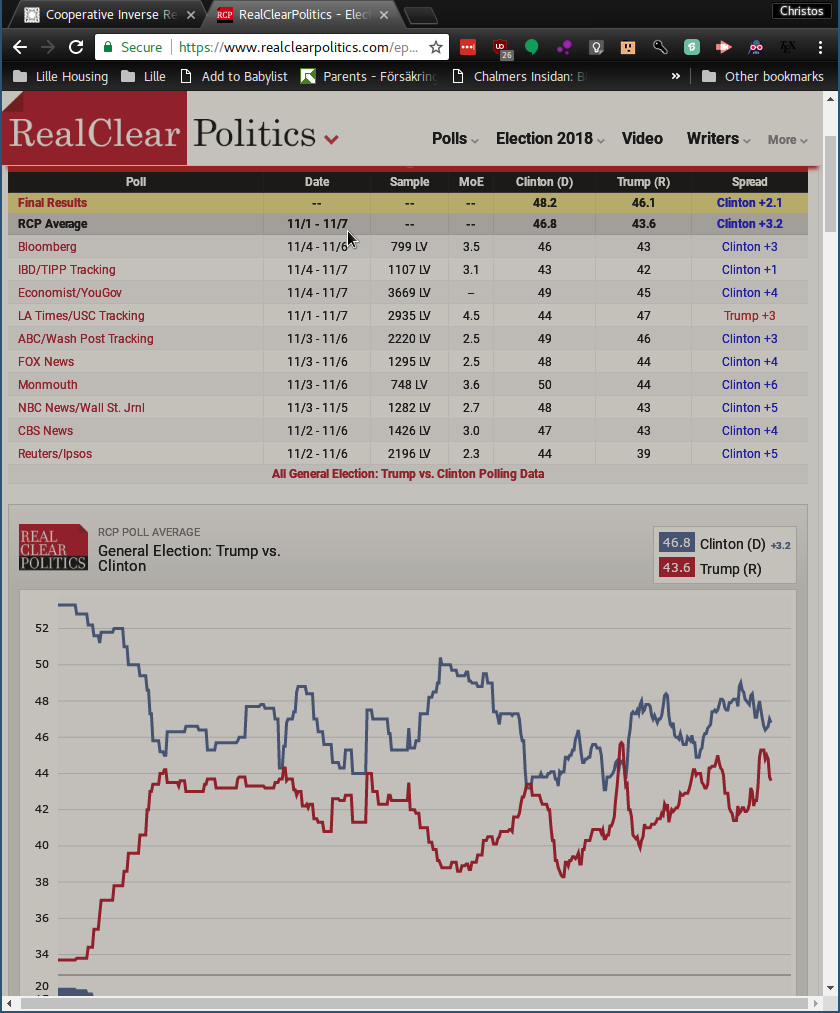
\includegraphics[width=\textwidth]{../figures/2016-election}}
\end{frame}

\subsection{Confidence intervals and $p$-values}
\begin{frame}
  \frametitle{The fallacy of $p$-values}
  \only<article>{A $p$-value has a uniform distribution under the null hypothesis. More precisely,let $x$ is our data and $H_0$ is our null hypothesis. If $H_0$ is true then $x \sim P_0$. Let}
  \[
    f(x) \tag{$p$-statistic}
  \]
  \only<article>{be a statistic on the data designed to have the property:}
  \[
    P_0(\cset{x}{f(x) \leq p}) = p.
  \]
  \only<article>{This ensures that the probability of rejecting the null hypothesis when it is true is actually $p$. But note that this is the definition of the uniform distribution, so $f(x)$ has a uniform distribution under $H_0$. Hence the value of $f(x)$ itself is uninformative. In theory we should simply choose $p$ before seeing the data and just accept or reject based on whether $f(x) \leq p$. However nobody does that in practice, meaning that $p$-values are used incorrectly. Better not to use them at all.}
\end{frame}


\begin{frame}
  \frametitle{Confidence intervals}
  \only<article>{Similarly, a confidence interval $I$ tells us the probability of an underlying value $\theta$ to be estimated being in $\theta \in I$, if our modelling assumption is correct.}
  \begin{block}[Confidence interval under a model $\mu$]
    \only<article>{
      The interval $I(\delta)$ for an estimator $\hat{\theta}$ of a parameter $\theta$ from data $x$ under the modelling assumptions $\mu$ is simply a set in $\Theta$ such that the true parameter lies in $I(\delta)$ with probability $1 - \delta$, i.e.
    }
    \[
      \Pr_\mu(\hat{\theta} \in I(\theta, \delta)) \geq 1 - \delta.
    \]
  \end{block}
  This is a property of the estimator $\hat{\theta} : \CX \to \Theta$ and tells us \emph{nothing direct} about our specific estimate $\hat{\theta(x)}$. \only<article>{It only tells that if we repeatedly apply this produre, we will only get an estimate outside of the interval a $\delta$-fraction of the time.}
\end{frame}

\subsection{Bayesian credible intervals}


\subsection{Model mismatch}

\subsection{Boot-strapping}

\subsection{Cross-validation}

\subsection{Independent replication}



%%% Local Variables:
%%% mode: latex
%%% TeX-master: "notes"
%%% End:

 


\bibliographystyle{plainnat}
\bibliography{../bibliography}

\end{document}
%%% Local Variables:
%%% mode: latex
%%% TeX-master: "notes"
%%% End:
